%%%%%%%%%%%%%%%%%%%%%%%%%%%%%%%%%%%%%%%%%%%%%%%%
%
% Strath PhD Thesis Template
%	by Jethro Browell [jethro.browell@strath.ac.uk]
%
%	Guidelines for thesis format, submission and content are found in
%	General and Course Regulations for Graduate and Postgraduate
%	Awards and Degrees, section 20.6.
%
%	Using .eps or .pdf is recomended to prduce high quality figures etc.
%
%	The Strathclyde logo can be found in other formats at www.strath.ac.uk.
%
%%%%%%%%%%%%%%%%%%%%%%%%%%%%%%%%%%%%%%%%%%%%%%%%

\documentclass[a4paper,oneside,11pt]{book}

% bold symbols
\newcommand{\betabb}{\boldsymbol{\beta}}
\newcommand{\nablabb}{\boldsymbol{\nabla}}
\newcommand{\gammabb}{\boldsymbol{\gamma}}
\newcommand{\sigmabb}{\boldsymbol{\sigma}}

% Pauli matrices
\newcommand{\sx}{\sigma^x}
\newcommand{\sy}{\sigma^y}
\newcommand{\sz}{\sigma^z}

% AGP-related commands
\newcommand{\dlambda}{\partial_{\lambda}}
\newcommand{\AGP}[1]{\mathcal{A}_{#1}}
\newcommand{\adj}[1]{#1^{\dagger}}
\newcommand{\dotlambda}{\dot{\lambda}}
\newcommand{\approxAGP}{\Bar{\AGP{\lambda}}}

% Other mathsy things
\newcommand{\HCD}{H_{\rm CD}}
\newcommand{\R}{\mathbb{R}}
\newcommand{\C}{\mathbb{C}}

% Formatting stuff + comments
\newcommand{\acrref}[1]{\hyperref[acr:#1]{#1}}
\newcommand{\reminder}[1]{\textcolor{blue}{Reminder: #1}}

% Some help with writing pseudocode
\makeatletter
\def\BState{\State\hskip-\ALG@thistlm}
\makeatother

\usepackage{amsbsy}
\usepackage{amsmath}
\usepackage{amsfonts}
\usepackage{graphicx}
\usepackage{multirow}
\usepackage{mathrsfs}
\usepackage{color}
\usepackage{xurl}
\usepackage[hidelinks]{hyperref}
\hypersetup{breaklinks=true}
\usepackage{cite}
\usepackage{enumitem}
\usepackage{epsfig}
\usepackage{caption}
\usepackage{subcaption}
\usepackage{physics}
\usepackage[strict]{changepage}
\usepackage{epigraph}
\usepackage{lipsum}
\usepackage{wrapfig}
\usepackage{algorithm}
\usepackage{algorithmicx}
\usepackage{algpseudocode}
%\usepackage{algcompatible}
\usepackage{mdframed}
\usepackage{cleveref}
\usepackage{dsfont}

\setcounter{secnumdepth}{5}

%own macros

% Page Margins - Strath Requirement
\usepackage[left=4cm,right=2.5cm,top=2cm,bottom=4cm,includehead,includefoot,headheight=15pt]{geometry}

\renewcommand\labelenumi{(\theenumi)}

% Page Headers
\usepackage{fancyhdr}
\fancyhf{}
\renewcommand{\headrulewidth}{0pt} % optional
%\fancyhead[L]{\nouppercase{\leftmark} \hfill Section \nouppercase{\rightmark}}
\fancyhead[L]{\nouppercase{\leftmark}}
\cfoot{\thepage}
\pagestyle{fancy}

% Draft Watermark
\usepackage[draft=true,allpages=true,fontfamily=cmr,angle=90,scale=0.1,mark={\fboxsep=35pt\fboxrule=0pt\relax\fbox{-- DRAFT -- \today~--}},xcoord=-80,ycoord=-20]{util/draftmark}

% Line Spacing
%\def\baselinestretch{1.5} 
\usepackage{setspace}
\setstretch{1.5}

\usepackage[most]{tcolorbox}
% new tcolorbox environment
% #1: tcolorbox options
% #2: color
% #3: box title

\newtcolorbox[auto counter,number within=section,crefname={box}{boxes}]{mycolorbox}[2][]{%
title=Box 1 $\mid$ Timeline, 
enhanced,
colback=PineGreen!10!white,
colframe=PineGreen!40!black,
colbacktitle=PineGreen!95!white,
fonttitle=\bfseries\upshape, 
code={\singlespacing},
subtitle style={boxrule=0.4pt},title=Box ~\thetcbcounter $\mid$ #2, label={#1}}

\newtcbtheorem[auto counter,number within=section]{theo}%
  {Theorem}{fonttitle=\bfseries\upshape, fontupper=\slshape,
     arc=0mm, colback=Periwinkle!10!white,colframe=Periwinkle!40!black,colbacktitle=Periwinkle!95!white}{theorem}


\usepackage{titling}
\pretitle{%
  \begin{center}
  \huge
  
\includegraphics[width=6cm]{images/logo}\\[\bigskipamount]
}
\posttitle{\end{center}}

%\title{Counterdiabatic, Better, Faster, Stronger: \\
%\Large{Overcoming Losses in Quantum Processes} \\ PhD Thesis}
\title{Fast \& Furious XXIII: \\
\Large{Counterdiabatic Optimised Local Driving} \\ PhD Thesis}
\author{Ieva \v{C}epait\.{e}
\\ \small Quantum Optics and Quantum Many-Body Physics\\[-0.8ex]
\small Department of Physics\\[-0.8ex]
\small University of Strathclyde, Glasgow\\
}

%%%%%%%%%%%%%%%%%%%%%%%%%%%%%%%%%%%%%%%%%%%%%%%%%%%%%%%%%%%%%%
\begin{document}

\maketitle

%%%%%%%%%%%%%%%%%%%%%%%%%%%%%%%%%%%%%%%%%%%%%%%%%%%%%%%%%%%%%%
\frontmatter
%%%%%%%%%%%%%%%%%%%%%%%%%%%%%%%%%%%%%%%%%%%%%%%%%%%%%%%%%%%%%%

% Declaration
\topskip0pt
\vspace*{\fill}
\noindent
\begin{quote}
	\centering
	This thesis is the result of the author's original research. It has been composed by the author and has not been previously submitted for examination which has led to the award of a degree. \\[5pt]
	%
	The copyright of this thesis belongs to the author under the terms of the United Kingdom Copyright Acts as qualified by University of Strathclyde Regulation 3.50. Due acknowledgement must always be made of the use of any material contained in, or derived from, this thesis. \\[5pt]
	%
	%Signed: \\
	%Date:
\end{quote}
\vspace*{\fill}
\chapter{Abstract}\label{chap:abstract}

Adiabatic protocols are employed across a variety of quantum technologies, from implementing state preparation and individual operations that are building blocks of larger devices, to higher-level protocols in quantum annealing and adiabatic quantum computation. The main drawback of adiabatic processes, however, is that they require prohibitively long timescales, leading to losses due to decoherence and heating. The problem of speeding up these processes while retaining the adiabatic condition has garnered a large amount of interest, resulting in a whole host of diverse methods and approaches that aim to do just that. Most of these are encompassed by the fields of quantum optimal control and shortcuts to adiabaticity (\acrref{STA}), which are in themselves complementary approaches. Optimal control concerns itself with control fields for steering system dynamics in the minimum allowed time, while the goal of \acrref{STA} is to retain the adiabatic condition upon speed-up.

This thesis is dedicated to the search for new ways to combine optimal control techniques with a universal method from \acrref{STA}: counterdiabatic driving or \acrref{CD}. The \acrref{CD} approach offers perfect suppression of all non-adiabatic effects experienced by a system driven by a time-dependent Hamiltonian regardless of how fast the process occurs. In practice, however, exact \acrref{CD} is difficult to derive often even more difficult to implement. The main result presented in the thesis is thus the development of a new method called counterdiabatic optimized local driving (\acrref{COLD}), which implements optimal control techniques in tandem with \emph{approximations} of exact \acrref{CD} in a way that maximises suppression of non-adiabatic effects. We show, using numerical methods, that using \acrref{COLD} results in a substantial improvement over optimal control or approximate \acrref{CD} techniques when applied to annealing protocols, state preparation schemes, entanglement generation, and population transfer on a synthetic lattice. We explore how \acrref{COLD} can be enhanced with existing advanced optimal control methods and we show this by using the chopped randomized basis method and gradient ascent pulse engineering. Furthermore, we demonstrate a new approach for the optimization of control fields that does not require access to the wave function or the computation of system dynamics. In their stead, we use components of the approximate counterdiabatic drive to inform the optimisation, owing to the fact that \acrref{CD} encodes information about non-adiabatic effects of a system for a given dynamical Hamiltonian. 

\tableofcontents

\chapter{Lay Summary}

At the moment, this is full of quotes from Star Trek I'd like to use:

\begin{itemize}
    \item "The slower you go, the more likely you'll get where you're going." - Stephen King, The Dark Tower
    \item "A library serves no purpose unless someone is using it." Mr. Atoz, "All Our Yesterdays"
    \item "Computers make excellent and efficient servants, but I have no wish to serve under them." Mr. Spock, "The Ultimate Computer"
    \item "Insufficient facts always invite danger." Mr. Spock, "Space Seed"
    \item "Change is the essential process of all existence." Mr. Spock, "Let That Be Your Last Battlefield"
    \item "Instruments register only through things they're designed to register. Space still contains infinite unknowns." Mr. Spock, "The Naked Time"
\end{itemize}

And now for some Terry Pratchett:

\begin{itemize}
    \item “Sometimes scientists change their minds. New developments cause a rethink. If this bothers you, consider how much damage is being done to the world by people for whom new developments do not cause a rethink.”
    \item “With magic, you can turn a frog into a prince. With science, you can turn a frog into a Ph.D and you still have the frog you started with.”
\end{itemize}
\chapter{Acknowledgements}

I would like to acknowledge that this was really really hard to put together and I need a break now.


\chapter{Acronyms and abbreviations}

\begin{table}[h]
      \begin{tabular}{p{3cm}  p{8cm}}

        \textbf{AGP}\label{acr:AGP} & Adiabatic Gauge Potential \\ [7pt]
        \textbf{ARP}\label{acr:ARP} & Adiabatic Rapid Passage \\ [7pt]
        \textbf{BDA}\label{acr:BDA} & Bare Dual Annealing \\[7pt]
        \textbf{BPO}\label{acr:BPO} & Bare Powell Optimisation \\[7pt]
        \textbf{CD}\label{acr:CD} & Counterdiabatic driving \\[7pt]
        \textbf{COLD}\label{acr:COLD} & Counterdiabatic Optimised Local Driving \\[7pt]
        \textbf{CRAB}\label{acr:CRAB} & Chopped Randomised Basis \\ [7pt]
        \textbf{GRAPE}\label{acr:GRAPE} & Gradient Ascent Pulse Engineering \\ [7pt]
        \textbf{GSA}\label{acr:GSA} & Generalized Simulated Annealing \\ [7pt]
        \textbf{LCD}\label{acr:LCD} & Local Counterdiabatic Driving \\[7pt]
        \textbf{PMP}\label{acr:PMP} & Pontryagin Maximum Principle \\[7pt]
        \textbf{QOCT}\label{acr:QOCT} & Quantum Optimal Control Theory \\[7pt]
        \textbf{STA}\label{acr:STA} & Shortcuts to Adiabaticity \\[7pt]

    \end{tabular}

\end{table}\label{table}

\addcontentsline{toc}{chapter}{List of Figures}
\listoffigures

%%%%%%%%%%%%%%%%%%%%%%%%%%%%%%%%%%%%%%%%%%%%%%%%%%%%%%%%%%%%%%
\makeatletter
\@mainmattertrue
\pagenumbering{arabic}
\makeatother
%%%%%%%%%%%%%%%%%%%%%%%%%%%%%%%%%%%%%%%%%%%%%%%%%%%%%%%%%%%%%%

\chapter{Introduction}


\section{Thesis overview}


\part{Background}
\chapter{Quantum Adiabaticity}\label{chap:2_adiabaticity}

\epigraph{I saw this movie about a bus that had to SPEED around a city, keeping its SPEED over fifty, and if its SPEED dropped, it would explode! I think it was called `The Bus That Couldn’t Slow Down'.}{Homer Simpson}

    
The concept of quantum adiabaticity is the central starting point of the work presented in this thesis. While in classical thermodynamics, an adiabatic process is essentially one where no heat or mass is transferred between a system and its environment, the quantum adiabatic theorem concerns itself more with the speed at which changes in a system Hamiltonian occur. The quantum adiabatic theorem, which I will explore in more detail in this chapter, states that \reminder{finish this}
        
    \section{The quantum adiabatic theorem}\label{sec:2.1_adiabatic_theorem}
    
    Imagine a quantum system that begins in the non-degenerate ground state of a time-dependent Hamiltonian. According to the the quantum adiabatic theorem, it will \emph{remain} in the instantaneous ground state provided the Hamiltonian changes sufficiently slowly. To take an intuitive example, we can consider a spin in a magnetic field that is rotated from the $x$ direction to the $z$ direction during some total time $\tau$. The Hamiltonian might be written as:
    \begin{equation}\label{eq:rotating_spin_H}
        H(t) = -\cos\Big(\frac{\pi t}{2 \tau}\Big)\sx - \sin \Big(\frac{\pi t}{2 \tau}\Big)\sz,
    \end{equation}
    where $\sx$ and $\sz$ are the Pauli matrices:
    \begin{equation}
        \sx = \mqty(0 & 1 \\ 1 & 0), \quad \sz = \mqty(1 & 0 \\ 0 & -1).  
    \end{equation}
    If the spin starts in the ground state of $H(0)$ (pointing in the $x$ direction, $\ket{\psi(0)} = \ket{+}$), then as the magnetic field is rotated, the spin starts precessing about the new direction of the field. This moves the spin toward the $z$ axis but also produces a component out of the $xz$ plane. As the total time for the rotation gets longer (\@i.e. the rotation gets slower compared to the precession), the state maintains a tighter and tighter orbit around the field direction. In the limit of $\tau \rightarrow \infty$, the state of the spin tracks the magnetic field perfectly, always in the ground state of $H(t)$ for all $t$. This is illustrated in Fig.~\ref{fig:bloch_rotating_spin} below, which shows the evolution of the system for increasing $\tau$ (and thus decreasing speed).
    
    \begin{figure}[h]
    \centering
    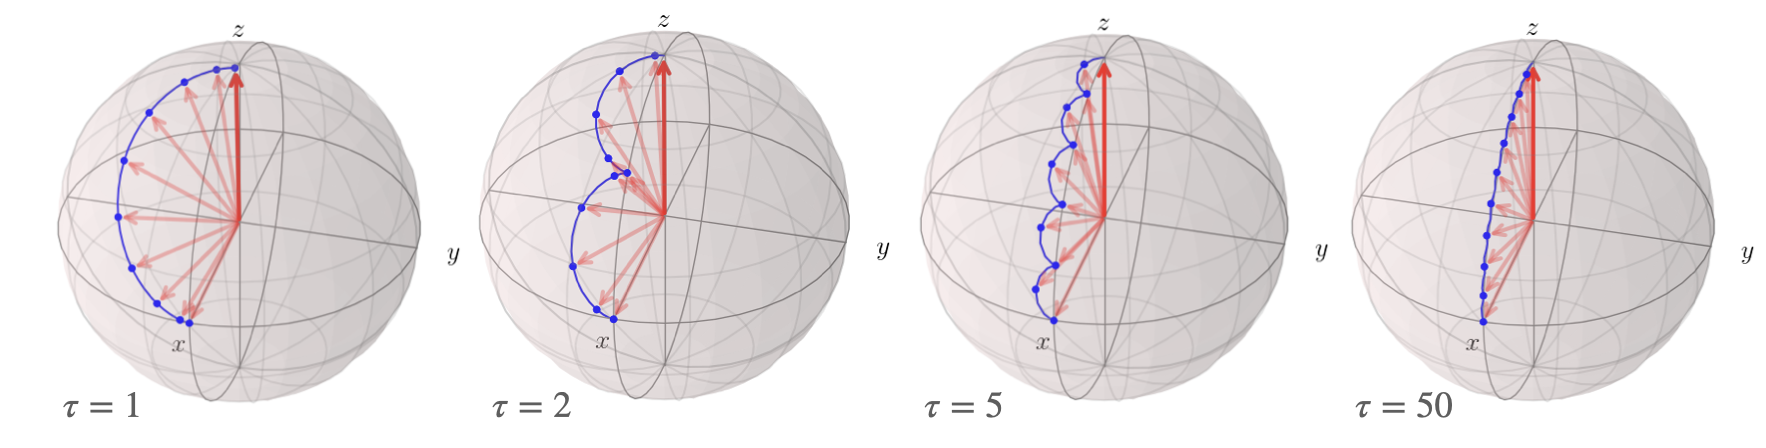
\includegraphics[width=0.9\linewidth]{images/magnetic_field_spin.png} \caption{Bloch sphere illustration of the single-spin system driven by the Hamiltonian of Eq.~\eqref{eq:rotating_spin_H} for different total driving times $\tau$.}\label{fig:bloch_rotating_spin}
    \end{figure}

    \subsection{Proof of the adiabatic theorem}\label{sec:2.1.1_proof_adiabatic_theorem}

    The above example gives some intuition for the behaviour of quantum systems as the time of evolution is slowed down, but it doesn't quite answer the question of what it means to be `slow enough' in the general case, ~\@i.e. what one would refer to as the \emph{adiabatic condition}. In order to characterise this regime, we first imagine a state $\psi(t)$ which evolves under some time-dependent Hamiltonian $H(t)$. For convenience, we redefine time through the parameter $\lambda = \frac{t}{\tau} \in [0,1]$, such that $\psi(t), H(t) \rightarrow \psi(\lambda), H(\lambda)$ vary smoothly as a function of $\lambda$. This is often done to capture the fact that there may be a natural parameterisation of the changing Hamiltonian such as, for example, two different angles describing a varying magnetic field, which we may want to explore. The parameter space we build generally has some geometric properties that relate to non-adiabatic effects, so it becomes important to talk about these abstract parameters instead of time. But more on this later!
    
    For each value of $\lambda$ throughout the evolution, we have a time-independent `instantaneous' Hamiltonian which can be diagonalised:
    \begin{equation}\label{eq:instantaneous_schroedinger}
        H(\lambda)\ket{n(\lambda)} = E_n(\lambda)\ket{n(\lambda)},
    \end{equation}
    where $E_n(\lambda)$ are the eigenenergies and $\ket{n(\lambda)}$ are the eigenvectors. Note that this is \emph{not} the time-dependent solution. The vectors $\ket{n(\lambda)}$ constitute a basis, so we can expand our quantum state at any value of $\lambda$ as:
    \begin{equation}\label{eq:adiabatic_basis_expansion}
        \ket{\psi(\lambda)} = \sum_n c_n(\lambda)e^{i \tau \theta_n(\lambda)}\ket{n(\lambda)},
    \end{equation}
    where $c(\lambda)$ are time-dependent coefficients through the parameter $\lambda$ and $e^{i \tau \theta_n(\lambda)}$ is the phase factor that an eigenstate picks up as a consequence of time-evolution with a time-independent Hamiltonian:
    \begin{equation}\label{eq:dynamical_phase}
        \theta_n(\lambda) = -\frac{1}{\hbar} \int_0^{\lambda} E_n(\lambda') d\lambda'.
    \end{equation}
    The factor of $\tau$ is simply a consequence of the change in variables $t \rightarrow \lambda$, since $\frac{d \lambda}{dt} = \dotlambda = \frac{1}{\tau}$.
    
    Thus, the task is now to solve the time-dependent Schr\"{o}dinger equation:
    \begin{equation}\label{eq:td-schroedinger}
        i\hbar \dotlambda \ket{\dlambda \psi(\lambda)} = H(\lambda) \ket{\psi(\lambda)},
    \end{equation}
    where $\dlambda$ is the partial derivative with respect to the parameter $\lambda$. We can then use the expansion Eq.~\eqref{eq:adiabatic_basis_expansion}, differentiate and take the inner product with some eigenstate $\bra{m(\lambda)}$ to get:
    \begin{equation}\label{eq:adiabatic_derivation}
        \begin{aligned}
         \frac{i\hbar}{\tau} \dlambda \sum_n c_n e^{i \tau \theta_n} \ket{n} &= H \sum_n c_n e^{i \tau \theta_n} \ket{n} \\
        \sum_n \Big( \dlambda c_n \ket{n} + c_n \ket{\dlambda n} + i \tau \dlambda\theta_n c_n \ket{n} \Big)e^{i \tau \theta_n} &= -\frac{i \tau}{\hbar} \sum_n E_n c_n e^{i \tau \theta_n} \ket{n} \\
        \sum_n \Big( \dlambda c_n \ket{n} + c_n \ket{\dlambda n} \Big)e^{i \tau \theta_n} &= 0 \\
        \dlambda c_m  &= - \sum_n c_n \braket{m}{\dlambda n}e^{i\tau(\theta_n-\theta_m)}
        \end{aligned}
    \end{equation}
    where the last two lines are a consequence of the fact that $i \tau \dlambda \theta_n(\lambda) = -\frac{i \tau}{\hbar} E_n(\lambda)$ and the the orthogonality of $\ket{m}$ and $\ket{n}$ when $m \neq n$. Note that I have removed the explicit dependence on $\lambda$ for the sake of readability and to make writing this all out more bearable and I will continue with this convention for the rest of the chapter unless otherwise stated. 
    
    The above differential equation is exact and describes the evolution of the coefficients $c_n$,  but it doesn't give much of a clue as to what `slow' time evolution means with respect to the changes in the Hamiltonian. For that, we can express the term $\braket{m}{\dlambda n}$ in terms of the changing Hamiltonian. This is done by differentiating Eq.~\eqref{eq:instantaneous_schroedinger} and then again taking the inner product with $\bra{m}$ to get:
    \begin{equation}\label{eq:hamiltonian_derivative}
        \begin{aligned}
            \dotlambda \Big(\dlambda{H}\ket{n} + H \ket{\dlambda n}\Big)  &= \dotlambda \Big(\dlambda{E_n}\ket{n} + E_n \ket{\dlambda n}\Big) \\
            \mel{m}{\dlambda H}{n} + \mel{m}{H}{\dlambda n} &= \dlambda E_n\braket{m}{n} + E_n \braket{m}{\dlambda n} \\
            E_m \braket{m}{\dlambda n} - E_n \braket{m}{\dlambda n} &= - \mel{m}{\dlambda H}{n} \\
            \braket{m}{\dlambda n} &= - \frac{\mel{m}{\dlambda H}{n}}{E_m - E_n}, \quad m \neq n
        \end{aligned}
    \end{equation}
    
    What the last line in Eq.~\eqref{eq:hamiltonian_derivative} shows is that we can express the term $\braket{m}{\dlambda n}$ in terms of the matrix components of $\dlambda H$ and the energy gap between the two eigenstates. If we plug this back into the final line of Eq.~\eqref{eq:adiabatic_derivation}, we find that:
    \begin{equation}\label{eq:coefficient_exact}
            \dlambda c_m -  c_m \braket{m}{\dlambda m} = \sum_{n \neq m} c_n  \frac{\mel{m}{\dlambda H}{n}}{E_m - E_n}e^{i \tau (\theta_n-\theta_m)}.
    \end{equation}
    When the term on the RHS is small we can neglect it and the solution for the remaining differential equation of $c_m$ is just:
    \begin{equation}\label{eq:c_adiabatic}
        c_m(\lambda) = c_m(0)e^{i \gamma_m(\lambda)},
    \end{equation}
    where:
    \begin{equation}\label{eq:geometric_phase}
        \gamma_m(\lambda) = i \int_0^{\lambda} \braket{m}{\partial_{\lambda'} m} d \lambda' 
    \end{equation}
    is the geometric (or Berry) phase \cite{pancharatnam_generalized_1956, longuet-higgins_studies_1958, berry_quantal_1984}. It arises from the fact that if the Hamiltonian varies according to $\lambda$ in a closed loop way, \@~i.e. it returns to its starting point at the end of the evolution, the wavefunction might not. Think Foucault's pendulum, which changes its plane of swinging due to the Earth's rotation around its own axis and does not necessarily return to its initial state after a full rotation! Both the appearance of the geometric phase in Eq.~\eqref{eq:c_adiabatic} and the changing plane of Foucault's pendulum are consequences of the geometry or `curvature' of the parameter space in which the dynamics occur and are related to concepts like parallel transport. \reminder{does this need citations? More elaboration?} 

    The constraint that the RHS of Eq.~\eqref{eq:coefficient_exact} be negligible is exactly the adiabatic condition, which can be seen by checking that $\abs{c_m(\lambda)}^2 = \abs{c_m(0)}^2$ in Eq.~\eqref{eq:c_adiabatic}. What this means is that a state starting in a particular eigenstate $\ket{m(\lambda)}$ will remain in that state under these circumstances, ~\@e.g. for $c_m(0) = 1$ and $c_{m \neq n}(0) = 0$:
    \begin{equation}\label{eq:adiabatic_states}
        \ket{\psi(\lambda)} = e^{i \tau \theta_m(\lambda)}e^{i \gamma_m(\lambda)} \ket{m(\lambda)}
    \end{equation}
    the $m^{\text{th}}$ eigenstate stays in the $m^{\text{th}}$ eigenstate.
    
    So to understand adiabaticity, we need to understand what conditions lead to the case where
    \begin{equation}\label{eq:adiabaticity_condition}
        \sum_{n \neq m} c_n \frac{\mel{m}{\dlambda H}{n}}{E_m - E_n}e^{i \tau (\theta_n-\theta_m)} \ll 1,
    \end{equation}
    which is exactly what the next section sets out to do.
    
    \subsection{The adiabatic condition: how slow is \emph{slow}?}\label{sec:2.1.2_adiabatic_condition}

    The condition given by Eq.~\eqref{eq:adiabaticity_condition} contains terms relating both to the rate of change of the Hamiltonian with respect to $\lambda$ (expressed in terms of matrix elements $\mel{m}{\dlambda H}{n}$) and the energy gap between eigenstates $E_m - E_n$. It is not too hard to see that when the energy gaps are very large, these terms can be neglected. However, let us try to derive a more concrete and quantitative measure for `slowness'.

    First, we can go back to the intermediate result from Eq.~\eqref{eq:coefficient_exact} and write it out as:
    \begin{equation}\label{eq:perturbative_adiabatic}
        \dlambda c_m = \sum_k c_k \frac{\mel{m}{\dlambda H}{k}}{E_m - E_k} e^{-\frac{i \tau}{\hbar}\int_0^{\lambda} E_m(\lambda') - E_k(\lambda') d\lambda'},
    \end{equation}
    where the exponential at the end is just a the dynamical phase from Eq.~\eqref{eq:dynamical_phase}. Let's again take the case that $c_n(\lambda) = 1$ and $c_{m \neq n}(\lambda) = 0$ at all values of $\lambda$, the approximate adiabatic solution. This leaves us with an equation which can be integrated:
    \begin{equation}\label{eq:nonadiabatic_perturbation}
        \begin{aligned}
            \dlambda c_{m \neq n} &= \frac{\mel{m}{\dlambda H}{n}}{E_m - E_n} e^{-\frac{i \tau }{\hbar}\int_0^{\lambda} E_m(\lambda') - E_n(\lambda') d\lambda'} \\
            \rightarrow c_{m \neq n} (1) &= \int_0^1 \frac{\mel{m}{\dlambda H}{n}}{E_m(\lambda) - E_n(\lambda)} e^{-\frac{i \tau }{\hbar}\int_0^{\lambda} E_m(\lambda') - E_n(\lambda') d\lambda'} d\lambda,
        \end{aligned}
    \end{equation}
    where, as already stated more than enough times, we expect the quantity $c_{m \neq n}$ to be $0$ (or as close to it as possible) for the adiabatic condition to hold. In fact, this was an assumption in the previous simplifying step! You can view these coefficients as the probabilities of transitioning out of the eigenstate $\ket{m}$ to the eigenstate $\ket{n}$ throughout the evolution. Since we'd like to keep our system in its initial (in this case $\ket{m}$) eigenstate at all times, it makes sense to minimise the RHS of Eq.~\eqref{eq:nonadiabatic_perturbation}. So, let us simplify the problem by first considering what are the quantities we can bound and where the largest contributions come from. In the case of the rate of change of the Hamiltonian, the largest matrix element will contribute more than the rest, so we can upper bound the contribution to the error via:
    \begin{equation}\label{eq:max_matrix_el}
        \max_{\ket{n(\lambda)}}\Big({\mel{m(\lambda)}{\dlambda H(\lambda)}{n(\lambda)}}\Big) \approx \overline{\mel{m}{\dlambda H}{n}}.
    \end{equation}
    The energy difference between the eigenstates in the denominator will have the largest impact when it is minimised (bearing in mind that this quantity is undefined if the two states are degenerate), so we can take the minimum possible energy gap as:
    \begin{equation}\label{eq:min_energy_diff}
        \min_{E_n(\lambda)} \Big(E_m(\lambda) - E_n(\lambda)\Big) = \overline{E_m - E_n}.
    \end{equation}
    With these two quantities in mind, we can now evaluate the last line of Eq.~\eqref{eq:nonadiabatic_perturbation} to find:
    \begin{equation}\label{eq:deriving_adiabatic_condition_final}
        \begin{aligned}
            c_{m \neq n} (1) &\approx \frac{\overline{\mel{m}{\dlambda H}{n}}}{\overline{E_m - E_n}} \int_0^1 e^{\frac{i \tau }{\hbar} \overline{E_m - E_n} \lambda} d \lambda \\
            &= \frac{i \hbar \overline{\mel{m}{\dlambda H}{n}}}{\tau(\overline{E_m - E_n})^2} \Big(e^{-\frac{i \tau }{\hbar}\overline{E_m - E_n}} - 1 \Big) \\
            &\approx \frac{i \hbar \dotlambda \overline{\mel{m}{\dlambda H}{n}}}{(\overline{E_m - E_n})^2},
        \end{aligned}
    \end{equation}
    where the final simplification is just due to the fact that the exponential term is oscillating with a maximum value of $1$. Since our goal is to bound $c_{m \neq n} (1)$ from above, we'll just set it to that maximum value. This leaves us with the simple criterion of what `slow' means with respect to the adiabatic regime:
    \begin{equation}\label{eq:adiabatic_criterion}
        \frac{i \hbar \dotlambda \overline{\mel{m}{\dlambda H}{n}}}{(\overline{E_m - E_n})^2} \ll 1, \quad m \neq n.
    \end{equation}

    In the example Hamiltonian of Eq.~\eqref{eq:rotating_spin_H}, the energy gap between its two eigenstates $\ket{\psi_1(t)}$ and $\ket{\psi_2(t)}$ is a constant: $E_{\psi_1} - E_{\psi_2} = 2$, and so are the matrix elements $\mel{\psi_1}{\dot{H}}{\psi_2} = \mel{\psi_2}{\dot{H}}{\psi_1} = \frac{\pi}{2 \tau}$. The dependence on $\tau$ of the off-diagonal matrix elements of $\dot{H}$ make the results of Fig.~\ref{fig:bloch_rotating_spin} immediately clearer: as $\tau$ increases (and hence the evolution is slower), the non-adiabatic component of Eq.~\eqref{eq:adiabatic_criterion} decreases proportionately to it. 

    I chose to elaborate on this proof in particular because it gave me a lot of intuition for what the adiabatic theorem \emph{is} and what I should look out for when I think of `slow' processes. In practice, however, it is not immediately obvious how the quantity stated in Eq.~\eqref{eq:adiabatic_criterion} relates to, say, the fidelity of the final state with respect to the desired state or how large $\tau$, the evolution time, has to be in order to lead to a fidelity of some magnitude. While it is possible to find these bounds, the proof is quite lengthy and not necessary for the purposes of this thesis, so instead I will refer you to \cite{reichardt_quantum_2004, childs_lecture_2008} for more details.
    
    \section{The adiabatic gauge potential}\label{sec:2.2_AGP}

    The previous section introduced quantum adiabaticity and presented some intuition for what non-adiabatic effects look like at fast driving times. In this section, I want to establish the deeply related concept of the adiabatic gauge potential (\acrref{AGP}) \cite{kolodrubetz_geometry_2017}, a key player in the subject matter of this thesis and a fascinating mathematical object in its own right. While the \acrref{AGP} has primarily been studied in the context of suppressing non-adiabatic effects \cite{sels_minimizing_2017, claeys_floquet-engineering_2019}, as will be its central role in this thesis, in recent years it has also been shown to be a potential probe for quantum chaos \cite{pandey_adiabatic_2020} and has been proposed for the study of thermalisation \cite{nandy_delayed_2022}. \reminder{add more here, mention ``geometric in nature"}

    \subsection{The moving frame Hamiltonian}

    In Section \ref{sec:2.1.1_proof_adiabatic_theorem} I spent a lot of time working in the instantaneous eigenbasis of the Hamiltonian where it is diagonalised, à la Eq.~\eqref{eq:instantaneous_schroedinger}. For a general Hamiltonian, it is possible to go to this `moving frame' picture by rotating the Hamiltonian via some unitary $U$ so that it becomes diagonal at each point in time. If we start with some arbitrary Hamiltonian $H(\lambda)$ in some sort of lab frame' that depends on time through the parameter(s) $\lambda(t)$, it can be diagonalised through $\Tilde{H} = U^{\dagger}(\lambda)H(\lambda)U(\lambda)$, where the $\sim$ implies that we are now in the basis of the moving frame and that the Hamiltonian is diagonal. In general, whenever the tilde symbol appears above an operator throughout this section, all it means is that we are working in this new basis: $\Tilde{\sigma} = \adj{U}\sigma U$.

    We can also view the quantum system evolving under the Hamiltonian in this moving frame picture: $\ket*{\Tilde{\psi}} = U^{\dagger}\ket{\psi}$, which is like expanding the wave function in the moving frame (or instantaneous) basis exactly as was done in Eq.~\eqref{eq:adiabatic_basis_expansion}. Given this new viewpoint, trying to solve the Schr\"{o}dinger equation, this time with the operators explicitly in mind, reveals something interesting:
    \begin{equation}\label{eq:moving_frame_schrodinger}
        \begin{aligned}
            i \hbar \frac{d \ket*{\Tilde{\psi}}}{dt} &= i \hbar \Big( \frac{d \adj{U}}{dt}\ket*{\psi} + \adj{U} \frac{d \ket{\psi}}{dt} \Big) \\
            &= i \hbar \dotlambda \frac{\partial \adj{U}}{\partial \lambda}\ket{\psi} + \adj{U} H\ket{\psi}\\
            &= \dotlambda \Big(i\hbar \frac{\partial \adj{U}}{\partial \lambda}U \Big)\ket*{\Tilde{\psi}} + \adj{U} H U \ket*{\Tilde{\psi}} \\
            &= \Big(\Tilde{H} - \dotlambda\Tilde{\AGP{\lambda}}\Big) \ket*{\Tilde{\psi}},
        \end{aligned}
    \end{equation}
    where the operator $\Tilde{\AGP{\lambda}}$ is the \emph{adiabatic gauge potential} with respect to the parameter $\lambda$ in the moving frame of the Hamiltonian $H$ and is expressed as:
    \begin{equation}\label{eq:AGP_in_terms_of_U}
        \Tilde{\AGP{\lambda}} = i\hbar \adj{U}\dlambda U.
    \end{equation}
    The name `gauge potential' generally refers to operators that are generators of continuous unitary translations in parameter space \cite{kolodrubetz_geometry_2017} of some unitary transformation $U$ and generally takes the form of a derivative operator. While there are many such gauge potentials out there, we'll restrict ourselves to the specific case of adiabaticity where the transformation $U(\lambda)$ explicitly takes a wavefunction in an arbitrary basis to the adiabatic or instantaneous basis. 
    
    So what we find is that the wavefunction in the moving frame basis evolves under a combination of the diagonal component $\Tilde{H}$ and some additional term proportional both to the speed at which the parameter $\lambda$ varies and the \acrref{AGP}. At this point I want to note that while there are $\sim$ symbols all over the place, we can actually apply the inverse unitary operation in order to work back in lab frame basis: $\Tilde{H} - \dotlambda\Tilde{\AGP{\lambda}} \xrightarrow{U \{ \cdot \} \adj{U}} H - \dotlambda \AGP{\lambda}$. In fact, this transformation makes it easy to see how we can think of the AGP in the lab frame as nothing more than the derivative operator: $\AGP{\lambda} = i\hbar\dlambda$. 

    To see this, take any quantum state written in some basis, \@~e.g. $\ket{\psi} = \sum_n \psi_n \ket{n}$. Then in the moving frame basis we have:
    \begin{equation}\label{eq:AGP_basis_change}
            \ket{\psi} = \sum_n \psi_n \adj{U}(\lambda) \ket{n} = \sum_{\Tilde{n}} \Tilde{\psi}_n (\lambda) \ket*{\Tilde{n}(\lambda)},
    \end{equation}
    where $\Tilde{\psi}_n (\lambda) = \sum_n \adj{U}(\lambda) \psi_n = \braket{\Tilde{n}(\lambda)}{\psi}$ and the dependence on $\lambda$ enters into the basis vectors through the rotation $U(\lambda)$. These two bases can now allow us to look at the matrix elements of $\AGP{\lambda}$ in both:
    \begin{equation}\label{eq:AGP_as_derivative}
        \begin{aligned}
            \mel{n}{\Tilde{\AGP{\lambda}}}{m} &= \mel{n}{i\hbar \adj{U}\dlambda U}{m} \\
            &= i\hbar \mel{\Tilde{n}(\lambda)}{\dlambda}{\Tilde{m}(\lambda)} \\
            &= \mel{\Tilde{n}(\lambda)}{\AGP{\lambda}}{\Tilde{m}(\lambda)}
        \end{aligned}
    \end{equation}
    where the last line is simply the statement that in the lab frame $\AGP{\lambda} = i\hbar \dlambda$.

    \subsection{Matrix elements of the \acrref{AGP}}

    What I've shown you so far is that when we try to solve the Schr\"{o}dinger equation for a quantum system evolving under a time-dependent Hamiltonian in the basis of the `moving frame', \@~i.e. in the basis where the time-dependent Hamiltonian is diagonalised, we find that the evolution happens under a `decorated' Hamiltonian with an additional operator that I've dubbed the adiabatic gauge potential or \acrref{AGP}. We found that in the lab frame, it is the derivative operator with respect to the time-dependent parameters driving the Hamiltonian. What remains is to link this to our discussion of adiabaticity and the adiabatic condition of Section \ref{sec:2.1_adiabatic_theorem}.

    Let us return to the matrix elements of the lab frame \acrref{AGP} and see what they are in the adiabatic basis of Eq.~\eqref{eq:instantaneous_schroedinger}, which is the eigenbasis of the instantaneous Hamiltonian. The first thing that jumps out is that the diagonal elements of the \acrref{AGP} are very familiar:
    \begin{equation}\label{eq:AGP_diagonal}
        \mel{n(\lambda)}{\AGP{\lambda}}{n(\lambda)} = i\hbar \mel{n(\lambda)}{\dlambda}{n(\lambda)}.
    \end{equation}
    The terms on the RHS are something known as the Berry connections and they look familiar because they are the integrands of the geometric phase (Eq.~\eqref{eq:geometric_phase}) that we found when deriving the adiabatic condition! I mentioned that the geometric phase is related to the geometry or `curvature' of the parameter space of the adiabatic Hamiltonian and it turns out that the \acrref{AGP} contains information about this geometry. 

    In order to understand what the off-diagonal elements of the AGP are, we can make use of the fact that in the instantaneous Hamiltonian basis $\mel{m}{H}{n} = 0$ for $m \neq n$. Differentiating with respect to the parameter $\lambda$ gives:
    \begin{equation}\label{eq:differentiating_adiabatic_offdiagonals}
       \begin{aligned}
           \mel{\dlambda m}{H}{n} + \mel{n}{\dlambda H}{n} + \mel{n}{H}{\dlambda m} &= 0 \\
           E_n \braket{\dlambda m}{n} + E_m \braket{m}{\dlambda n} + \mel{n}{\dlambda H}{n} &= 0 \\
           (E_m - E_n) \braket{m}{\dlambda n} + \mel{n}{\dlambda H}{n} &= 0 \\
           \frac{-i}{\hbar} (E_m - E_n) \mel{m}{\AGP{\lambda}}{n} + \mel{n}{\dlambda H}{n} &= 0 \\
           \mel{m}{\AGP{\lambda}}{n} &= i\hbar \frac{\mel{m}{\dlambda H}{n}}{(E_n - E_m)}
       \end{aligned} 
    \end{equation}
    where I'll stress again that since we're working in the adiabatic basis, all eigenstates, eigenenergies and the operators depend on $\lambda$. The final line is familiar: the off-diagonal elements of the \acrref{AGP} are proportional to the non-adiabatic contribution we derived back in Eq.~\eqref{eq:deriving_adiabatic_condition_final}. The full operator in the adiabatic basis is:
    \begin{equation}\label{eq:AGP_adiabatic_basis}
        \AGP{\lambda} = i\hbar\Big(\sum_n \braket{n}{\dlambda n} \dyad{n} + \sum_{m \neq n} \ket{m} \frac{\mel{m}{\dlambda H}{n}}{(E_n - E_m)} \bra{n} \Big)
    \end{equation}

    The outcome of this section then, is the revelation that this (initially mysterious) operator known as the \acrref{AGP} is deeply linked to the notion of adiabaticity in quantum systems: its diagonal terms are related to the geometry of the parameter space of adiabatic dynamics while its off-diagonals elements describe the non-adiabatic effects experienced by a state when it is driven by a time-dependent Hamiltonian. It is useful to note that in the final line of Eq.~\eqref{eq:moving_frame_schrodinger} we found that the Schr\"{o}dinger equation corresponding to the evolution of the instantaneous eigenstates is:
    \begin{equation}\label{eq:schrodinger_moving_frame_2}
        i \hbar \frac{d \ket*{\Tilde{\psi}}}{dt} = \Big( \Tilde{H} - \dotlambda \AGP{\lambda} \Big) \ket*{\Tilde{\psi}},
    \end{equation}
    where now it is not difficult to find how each of these operators contributes to the results of Section \ref{sec:2.1.1_proof_adiabatic_theorem}. The moving frame or instantaneous Hamiltonian generates the dynamical phase factor in Eq.~\eqref{eq:dynamical_phase}, the diagonal elements of the \acrref{AGP} produce the geometric phase factor given by Eq.~\eqref{eq:geometric_phase} and the off-diagonal elements of \acrref{AGP} are responsible for the non-adiabatic transitions out of the eigenstates which we upper bounded in Section \ref{sec:2.1.2_adiabatic_condition}. For a more detailed proof of how to derive the adiabatic theorem starting from Eq.~\eqref{eq:schrodinger_moving_frame_2} I recommend \cite{petiziol_accelerated_2020}. \reminder{Shall I include the proof in the Appendix instead? It's quite long but maybe it's nice to have for a bit of context.}
    
    \section{Counterdiabatic Driving}\label{sec:2.3_CD}

    Having done all this work to characterise and understand the \acrref{AGP} and the adiabatic theorem, we now come to a very important question which defines just about the entirety of this thesis: \emph{why do we care}? What is it about adiabatic dynamics and quantifying non-adiabatic transformations and understanding what generates them important? The answer is simple: adiabatic processes are useful. The ability to drive a time-dependent Hamiltonian while remaining in a some eigenstate of the system is something that can be used to prepare interesting quantum states \cite{dimitrova_many-body_2022}, to solve combinatorics problems encoded in quantum systems \cite{ebadi_quantum_2022, pichler_quantum_2018} or even to synthesise effective ramps and quantum logic gates \cite{pelegri_high-fidelity_2022} among many other applications. 
    
    The most natural way of exploiting adiabatic protocols is by adhering to the adiabatic condition. However, as is often the case when it come to the control of quantum systems, nothing is quite that simple. In practice, changing a Hamiltonian slowly enough to satisfy Eq.~\eqref{eq:adiabatic_criterion} leads to a system being overwhelmed by decoherence instead. Furthermore, as system sizes get larger, the energy gaps between the instantaneous eigenstates tend to get smaller \reminder{does this need a citation?} requiring slower and slower driving, making the scaling up of adiabatic protocols a big problem. The result, inevitably, is that we need to find ways to achieve the same results as adiabatic processes but without requiring the prohibitively long driving times that are demanded by Eq.~\eqref{eq:adiabatic_criterion}.
    
    

    \begin{equation}\label{eq:CD_Hamiltonian}
    H_{CD}(\lambda) = H(\lambda) + \dotlambda \mathcal{A}_\lambda,
    \end{equation}

    \subsection{The problem: finding the \acrref{AGP}}

    \subsection{A classic(al) analogy: the waiter and the glass of water}

    I will take a brief detour away from all the mathematics involved in 
    
    \subsection{Transitionless Driving}
    The form of the dynamical Hamiltonian enforcing this is \cite{berry_transitionless_2009}:
    \begin{equation}\label{eq:counterdiabatic}
        H_{\mathrm{CD}}(t) = H_0 (t) + i\hbar \sum_n (\ket{\partial_t n}\bra{n} - \bra{n}\ket{\partial_t n}\ket{n}\bra{n}),
    \end{equation}
    \subsection{Variational counterdiabatic driving}

    \begin{equation}\label{eq:energy_derivative}
        \begin{aligned}
            \frac{dE}{dt} &= \frac{d}{dt}\ev*{\Tilde{H}}{\Tilde{\psi}} \\
            &= \dotlambda \ev*{\dlambda \Tilde{H}}{\Tilde{\psi}} - \frac{i}{\hbar} \dotlambda \ev*{\comm*{\Tilde{\AGP{\lambda}}}{\Tilde{H}}}{\Tilde{\psi}} \\
            &= -\dotlambda F_{\lambda} - \frac{i}{\hbar} \dotlambda \ev{\comm{\AGP{\lambda}}{H}}{\psi},
        \end{aligned}
    \end{equation}
    where the commutator in the second line appears because $i\hbar d_t \ket*{\Tilde{\psi}} = (\Tilde{H} - \dotlambda\Tilde{\AGP{\lambda}}) \ket*{\Tilde{\psi}}$
    
    Following the methods of Ref.~\cite{sels_minimizing_2017}, the problem of finding the optimal adiabatic gauge potential can be cast as the minimisation of the Hilbert-Schmidt norm of the operators
    \begin{equation}\label{eq:Goperator}
     G_{\lambda}= \dlambda H_\beta + i\comm{\mathcal{A}_\lambda}{H_\beta},
    \end{equation}
    which is equivalent to minimisation of the action
    \begin{equation}\label{eq:actionCD}
    \mathcal{S}(\mathcal{A}_{\lambda}) = \Trace{\left[G_{\lambda}(\mathcal{A}_{\lambda})^2\right]},
    \end{equation}
    with respect to $\mathcal{A}_{\lambda}$.
    \subsection{Nested commutator expansion}
    \subsection{Krylov methods}

    \subsection{Shortcuts to adiabaticity}
    
    Here I'm going to talk about Shortcuts to Adiabaticity 
    (\acrref{STA})

\chapter{Quantum Optimal Control}\label{chap:3_Quantum_Optimal_control}
\epigraph{``Neo, sooner or later you’re going to realize, just as I did, that there’s a difference between knowing the path and walking the path."}{Morpheus, \emph{The Matrix (1999)}}

The future of quantum technologies depends on our ability to control quantum systems with precision and accuracy. It is a key factor in the realisaton of, for example, quantum computers \cite{ball_software_2021}, communication systems \cite{omran_generation_2019} and quantum sensors \cite{le_robust_2021}, as well as being necessary in the exploration and understanding of fundamental physics. The research field which concerns itself with such control problems is generally known as Quantum Optimal Control Theory (\acrref{QOCT}) \cite{koch_quantum_2022,glaser_training_2015} and its primary objective is the development of techniques which allow for the construction and analysis of strategies, primarily electromagnetic field shapes, that manipulate quantum dynamical processes in the most efficient and effective way possible in order to achieve certain objectives. Common control objectives in the quantum setting can range from state preparation \cite{zhang_when_2019} and quantum gate synthesis \cite{pelegri_high-fidelity_2022}, to protection against decoherence \cite{rooney_decoherence_2012} and entanglement generation \cite{omran_generation_2019}.

While the field of quantum optimal control is vast and would take an entire book to summarize \cite{dalessio_quantum_2016}, this chapter aims to give a broad overview of the topic highlighting its structure, mechanisms, and practical applications, in particular with respect to the methods that are relevant to the rest of the work presented in this thesis. As such, in Sec.~\ref{sec:3.1_structure_quantum_control}, we will begin by exploring the general structure of optimal control problems in detail and showing how an abstract goal can be transformed into a quantitative formula that guides us towards some desired outcome satisfying a given control objective. First, we will discuss the mathematical structure of optimal control problems (Sec.~\ref{sec:3.1.1_mathematical_structure}) followed by an overview and examples of analytical (Sec.~\ref{sec:3.1.2_analytic_optimisation}) and numerical (Sec.~\ref{sec:3.1.3_numerical_optimisation}) methods for finding solutions to said problems, with a focus on methods that will be relevant to the rest of the content in this thesis. Sec.~\ref{sec:3.2_Quantum_optimal_control} will review how optimal control is adapted in the quantum setting and the main idea behind \acrref{QOCT}, while Sec.~\ref{sec:3.3_qoct_methods} will focus on specific methods used for constructing and optimising driving pulses with quantum systems in mind.

\section{The structure of optimal control problems}\label{sec:3.1_structure_quantum_control}

The idea of an optimal control problem is simple: envision a target you want to achieve, cast it into some form of quantitative or abstract mathematical formula and then use this formula to derive the `best' path to get to said objective. There may be many paths to achieve the target and there may be many metrics to determine what `best' means. The aim of the first part of this section is thus to broadly cover the mathematical structure of optimal control problems and to try and convey an idea of what an optimal path \emph{is} and how one might quantify its optimality. Later in the chapter, we will delve more into practical questions of controllability and the process of optimisation, \@i.e.~once an optimal control problem is constructed, how does one go about finding the solution to it. We will cover both analytical methods in Sec.~\ref{sec:3.1.2_analytic_optimisation} and numerical approaches in Sec.~\ref{sec:3.1.3_numerical_optimisation} focusing on a select few optimisation algorithms which will be relevant to further chapters of this thesis. 

\subsection{Mathematical structure}\label{sec:3.1.1_mathematical_structure}

In general, an optimal control problem is composed of a set of state functions $X: \R \rightarrow \R^n$, and a set of time-dependent control functions $U:\R \rightarrow \R^m$ and the optimal control problem consists of finding $x \in X$ and $u \in U$ that minimise some functional $C: X \cross U \rightarrow \R$ such that the constraint
\begin{equation}\label{eq:control_ODE}
    \dot{x} = f(x, u),
\end{equation}
is satisfied almost everywhere. This is a very abstract description and just about any control problem can be expressed as a special case of this formulation \cite{dalessandro_introduction_2021}. To gain more intuition, we can imagine a more concrete example where, \@e.g.~$U$ and $X$ are sets of continuous functions on the interval $[0, \tau]$ satisfying $x(0) = x_0$. In this scenario, $\tau$ could be a time interval during which we want to drive the system from an initial state $x_0$ to a final state $x_f$ using the control function $u(t)$, $t \in [0, \tau]$. The choice of functional $C$ would have to capture the desired outcome of the protocol: that the state of the system after the driving $x(\tau)$ be equal to the target $x_f$. This can be done by choosing a distance metric that depends on only on the drive $u$ and is minimised when $x(\tau) = x_f$, \@~e.g.
\begin{equation}\label{eq:example_cost_func}
    C(u) = \norm{x(\tau)  - x_f}^2.
\end{equation}
The functional $C$ is often referred to in literature as the \emph{cost} or \emph{loss} function \cite{wald_statistical_1950} as it encodes the quality of the final protocol with respect to the desired outcome of the protocol. In that sense, we can imagine adding constraints to the problem that may increase the `cost' of the protocol output if they are not satisfied to some degree. For example, Eq.~\eqref{eq:example_cost_func} can be modified to include additional terms:
\begin{equation}\label{eq:example_cost_func2}
    C(u) = \gamma \norm{x(\tau)  - x_f}^2 + \int_0^{\tau} \norm{u(t)}^2 dt,
\end{equation}
where $\gamma$ is a penalty term on the final state that scales its importance relative to the additional second term, which is analogous to the cost in the energy required to achieve the final state. This updated cost function can be read as introducing a competition between the quality of the final state and the amount of energy expended to get it there, mediated by the value of $\gamma$. 

\begin{figure}[t]
\centering
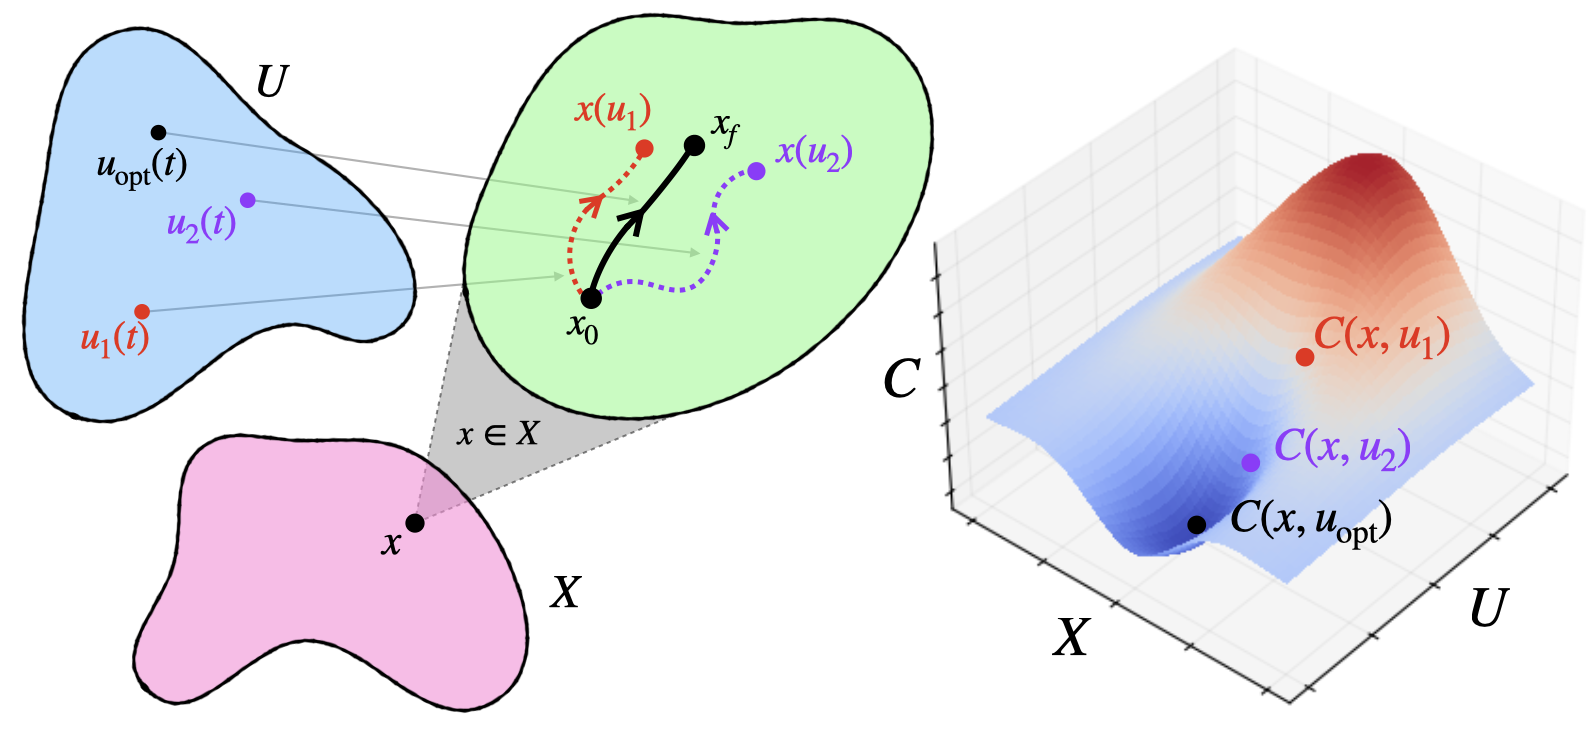
\includegraphics[width=0.9\linewidth]{images/optimal_control_illustration.png} \caption[Illustration of optimal control problem structure]{Illustration of the Mayer type optimal control problem: when an initial value of the system state $x_0$ is fixed, the choice of control function $u \in U$ and the requirement of satisfying Eq.~\eqref{eq:control_ODE} determine $x$ uniquely. The task is then to find $u_{\rm opt}$ such that the functional $C(x, u_{\rm opt})$ is minimised.}\label{fig:optimal_control}
\end{figure}

There are primarily three different types of problem structures in optimal control centering on different constraints and targets: \emph{Mayer-type}, \emph{Lagrange-type} and their combination, \emph{Bolza} problems \cite{dalessandro_introduction_2021}. In this thesis, we will mostly focus on Mayer-type problems, particularly in Ch.~\ref{chap:4_COLD} and Ch.~\ref{chap:6_Applications_fidelity}. In Mayer problems, the initial state is specified $x(0) = x_0$ and the cost function is of the form
\begin{equation}\label{eq:mayer_costfunc}
    C(u) = \phi(x(\tau), \tau),
\end{equation}
with $\phi$ a smooth function and $\tau$ the total time of the protocol. These two constraints and the requirement given by Eq.~\eqref{eq:control_ODE} define the state function $x$ uniquely and the problem is then to determine a control function $u$ on the appropriate set $[0, \tau]$ which minimises Eq.~\eqref{eq:mayer_costfunc}. In Mayer-type problems, a specific target state can be defined in the cost function as a constraint, which is the case in Eq.~\eqref{eq:example_cost_func} and this is illustrated in Fig.~\ref{fig:optimal_control}. However, this need not be the case as target states can be made implicit by having the cost function target some property of the state instead, like Euclidean distance from the initial state in the case of real vectors over Cartesian coordinates. 

From the above, we can view Mayer-type problems as being concerned primarily with the final state of the system and not its path. Lagrange-type problems, on the other hand, put focus on the behaviour of the system throughout the control trajectory and they encompass cost functions of the type
\begin{equation}\label{eq:lagrange_type_costfunc}
    C(u) = \int_0^{\tau} L(x, u, t) dt,
\end{equation}
where $L$ is a smooth function. This type of cost function is applicable, for example, in cases where one wants to minimise the expenditure of some path-dependent resource during the control procedure, or where a path-dependent quantity is easier to optimise over than a target state quantity. This type of optimisation is something that will become relevant in Ch.~\ref{chap:5_cd_as_costfunc} and Ch.~\ref{chap:7_higher_order_agp}. 

The most general type of problem is the Bolza problem, which combines both Mayer and Lagrange in a way that puts emphasis both on the target state of the optimal control and the trajectory that a system takes to get there:
\begin{equation}\label{eq:bolza_tyoe_costfunc}
    C(u) = \phi(x(\tau), \tau) + \int_0^{\tau} L(x, u, t) dt,
\end{equation}
where $\phi$ and $L$ are smooth functions given in Eq.~\eqref{eq:mayer_costfunc} a. A great example of Bolza-type problems is the cost function given by Eq.~\eqref{eq:example_cost_func2}, which comprises a competition between distance to a target state and the energy expended to drive the system to said state. 

Apart from identifying the basic anatomy of control problems in terms of $X$, $U$ and $C$, there is a myriad of additional information about their mathematical structure that can help to analyse and thus solve them. For example, it might be useful to identify if, for a particular optimal control problem, the system in question is \emph{controllable}\cite{dirr_lie_2008, fleming_optimal_1975} \@i.e.~can any initial state be transformed into any desired target state. Equally, it might be useful to study what are called \emph{reachable sets}\cite{vom_ende_reachability_2020, fleming_optimal_1975}, which are sets containing all the states that an initial state can be driven to by the set of control functions $U$. In the case of Mayer-type problems, for example, it might be sensible to define a reachable set parameterised by the final evolution time $\tau$ such that it contains all possible states that can be obtained by the system during a driving time $\tau$. Finally, it would be remiss not to mention the concept of \emph{necessary conditions for optimality}\cite{mangasarian_sufficient_1966}, which focus on determining what formal conditions need to be satisfied for a specific control $u \in U$ to be optimal. Generally, this involves perturbing an assumed optimal control $u$ by some small parameter $\epsilon$ giving $u^{\epsilon}$ and then imposing the constraint that
\begin{equation}\label{eq:optimality_condition}
    C(u^{\epsilon}) - C(u) \geq 0,
\end{equation}
which is then considered the necessary condition for optimality. The most basic of these optimality conditions is the Pontryagin maximum principle or \acrref{PMP} \cite{boltyanski_nonclassical_1999} (see Appendix \ref{app:PMP}), which states that for an optimal control problem, the optimal control and state trajectories should maximize a specific function which combines the system dynamics, the control inputs, and the Lagrange multipliers which encode the constraints of the control problem.

\subsection{Analytical optimisation}\label{sec:3.1.2_analytic_optimisation}

While the first part of optimal control is the construction of the problem, the second part is the search for a solution. The methods used to do this can generally be classified either as analytical or numerical approaches. While both are widely used in optimal control theory, this thesis will largely only focus on the latter, as such we will be brief in introducing the former. 

Analytical optimal control techniques are those that leverage mathematical rigor and formalism to derive solutions or insights, as opposed to relying primarily on numerical simulations, heuristics, or experimentation. They provide a theoretical foundation for understanding the properties and solutions of optimal control problems and are closely related to the discussion in Sec.~\ref{sec:3.1.1_mathematical_structure}. They can allow for a complete geometric understanding of the control problem leading to, for example, knowledge of the structure of a solution or even some proof about a global optimum. For a given set of constraints they might even be used to derive time limits of state transformations, \@i.e.~the concept of reachability. An example of analytical methods is the aforementioned \acrref{PMP}, which provides information about the optimal solution by via a set of differential equations. A different analytical control theory tool, the Hamilton-Jacobi-Bellman equation \cite{yong_dynamic_1999}, provides a way to find the optimal protocol via dynamic programming\cite{sniedovich_dynamic_2010}.

The trouble with analytical approaches, despite the commonplace rigorous guarantees of optimality and the scope of information they provide about the system, trajectory and structure of the control problems and their solutions, is that they are very difficult to scale up and quite inflexible to complex problem constraints. As such, analytical approaches are generally reserved for special cases, when problems have low dimensionality and simple structures where the cost function is generally linear in the arguments. Many real-world control systems require more complexity and flexibility than can be afforded by analytical methods.

\subsection{Numerical optimisation}\label{sec:3.1.3_numerical_optimisation}

To overcome the drawbacks of analytical approaches, many optimal control problems are instead solved using numerical optimisation methods. These are generally algorithmic, iterative  techniques which explore the cost function landscape step-by-step in order to converge to a minimum value. Numerical methods, as a general rule, do not offer the same analysis or guarantees of optimality that analytical methods do. Their iterative nature may lead to a dependence of the outcome on the initial conditions of the algorithm, such as an initial guess for an optimal solution from which the iterations proceed or the bounds on the search space. Despite these drawbacks, however, numerical methods tend to be far more popular than analytical ones simply due to their flexibility and applicability. Where analytical approaches fail, the only way forward is often a numerical method.

A general numerical optimisation technique consists of an initialisation step, a series of search steps and a termination step. These can be summarised as follows:
\begin{enumerate}
    \item \emph{Initialisation}: set up the necessary constraints of the optimal control problem, such as bounds on the solution space or an initial guess for the optimal solution.
    \item \emph{Search}: Perform some iterative search steps (deterministic or stochastic) with the goal of converging to the minimum of the cost function. What constitutes a single step varies massively between different techniques.
    \item \emph{Termination}: Return a solution after some condition is satisfied. This can be a convergence criterion based on the change in the cost function value between steps or a limit on the number of search steps that the algorithm is allowed to perform.
\end{enumerate}

The simplicity of these three components leaves a lot of room for creativity and over the years many numerical optimisation algorithms and techniques have been developed to deal with different constraints and topologies of different cost function landscapes. It would take an entire book \cite{nocedal_numerical_2006} to cover the various categories and subcategories that exist within the field, so I will restrict myself to exploring a few key classifications of the structure of numerical optimisation methods. 

One of the more broad ways to classify numerical optimisation methods is into the categories of \emph{gradient-based} methods and \emph{gradient-free} methods. Gradient-based methods, as the name implies, make use of gradient information (the first derivative of the cost function) to guide the search for an optimal solution. These methods are often efficient and converge rapidly when the cost function is smooth and differentiable. A popular example of a gradient-based method is the gradient descent algorithm, which iteratively adjusts the solution in the direction opposite to the gradient, as this direction is likely the steepest decrease in the cost function value. A typical gradient descent protocol might look like:
\begin{equation}\label{eq:gradient_descent}
    \ubb_{n + 1} = \ubb_n - \mu \grad_{\ubb} C(\ubb_n),
\end{equation}
where $n$ denotes the current iteration of the algorithm, $\grad_{\ubb} C(\ubb_n)$ is the derivative of the cost function $C$ with respect to the control parameters $\ubb$ and $\mu$ is generally known as the `learning rate' or `step size' and its job is to control the resolution at which the algorithm traverses the cost landscape. Larger $\mu$ might lead to faster convergence but it might also mean overshooting the cost function minimum, so adjusting its value is often a heuristic that requires some experimentation. Other examples of gradient-based methods include Newton's method and quasi-Newton methods \cite{suli_introduction_2003}, which employ information about the second derivative to guide the search and provide faster convergence as well as a myriad of other approaches including stochastic methods \cite{bottou_tradeoffs_2007}. 

Gradient-free methods, on the other hand, do not require gradient information, making them suitable for optimization problems where the cost function is, \@e.g.~ discontinuous, non-differentiable, or its gradient is difficult or expensive to compute. Examples of gradient-free methods include particle swarm optimization\cite{bonyadi_particle_2017}, the Nelder-Mead method, which I will explore in more detail in Sec.~\ref{sec:3.1.3.1_Nelder_Mead} as well as the Powell method of Sec.~\ref{sec:3.1.3.2_Powell}. These methods often rely on trial and error, random sampling, or mimicking natural phenomena like evolutionary mechanisms\cite{vikhar_evolutionary_2016} to explore the solution space. As in the case of gradient-based approaches, there is a veritable zoo of methods under this umbrella. As the rest of this thesis we will deal almost exclusively with gradient-free methods, I will provide examples of how these techniques look in the next couple of sections.

Apart from the gradient-information, another key way to classify optimisation algorithms is either as \emph{local} or \emph{global}. Local optimization methods are designed to find a local minimum, which is a solution that is better than all other feasible solutions in its vicinity in the landscape of the cost function. They are typically efficient at converging to the local minimum, but they provide no guarantee of finding the global minimum if the cost function is non-convex \@i.e.~the local minimum is not automatically also the global minimum. Both Nelder-Mead and Powell are local methods.

Global optimization methods, on the other hand, aim to find a global optimum, which is the best solution among all feasible solutions, not just those in a local neighborhood. These methods typically employ a strategy to explore the entire solution space, either deterministically or stochastically, to avoid getting trapped in a local optimum. As a result of this larger scope, global optimization methods are generally more computationally intensive than local methods. An example of global optimisation that I will explore in more detail in Sec.~\ref{sec:3.1.3.3_dual_annealing} is Dual-Annealing, which combines generalized simulated annealing\cite{tsallis_generalized_1996}, a global search algorithm, with local optimisers in order to find an optimal solution. Global methods are often used when the optimization problem is complex, non-convex, or the global solution is significantly better than any local solution.

Finally, in numerical optimal control we can make a distinction between open-loop and closed-loop optimisation, particularly when referring to the real-life use or experiments on a given system:
\begin{itemize}
    \item \emph{Open-loop} approaches calculate the control sequence ahead of time and apply it to the system irrespective of the system's actual behavior during the protocol. 
    \item \emph{Closed-loop} methods actively adjust the control strategy based on the current and past states of the system (see Fig.~\ref{fig:quantum_optimal_control}).
\end{itemize}
The closed loop approach is more resilient to uncertainties and disturbances but requires real-time computation or pre-computed feedback laws. In this thesis, the focus will be exclusively on open-loop approaches, as closed-loop methods require access to live experimental data which was not available in the case of the methods explored in later chapters. However, it is important to acknowledge that the results obtained in open-loop optimisations may not reflect the realistic, complex response a physical system might have to a specific control protocol, given that the model we use may not include the full details of the physical system. 

In the following sections I give examples of some common numerical optimisation methods that were used to obtain the results presented in this thesis.

\subsubsection{Nelder-Mead}\label{sec:3.1.3.1_Nelder_Mead}

A frequently used gradient-free optimisers is the Nelder-Mead (or downhill-simplex) method \cite{nelder_simplex_1965} developed by J. Nelder and R. Mead in 1965. It is referred to as a \emph{direct search} or \emph{pattern search} approach and it is a gradient-free local method, making it generally quite efficient, but not guaranteed to converge to a global optimum of the cost function. Direct search methods work by varying each optimisable parameter by some small stepsize from the current minimum in each direction and computing the cost function at the updated value. The change that leads to the largest decrease in the cost function value is taken as the new minimum. Once no such variation leads to an improvement, the stepsize is halved and the process is repeated until some convergence criterion is satisfied.

\begin{figure}[t]
\centering
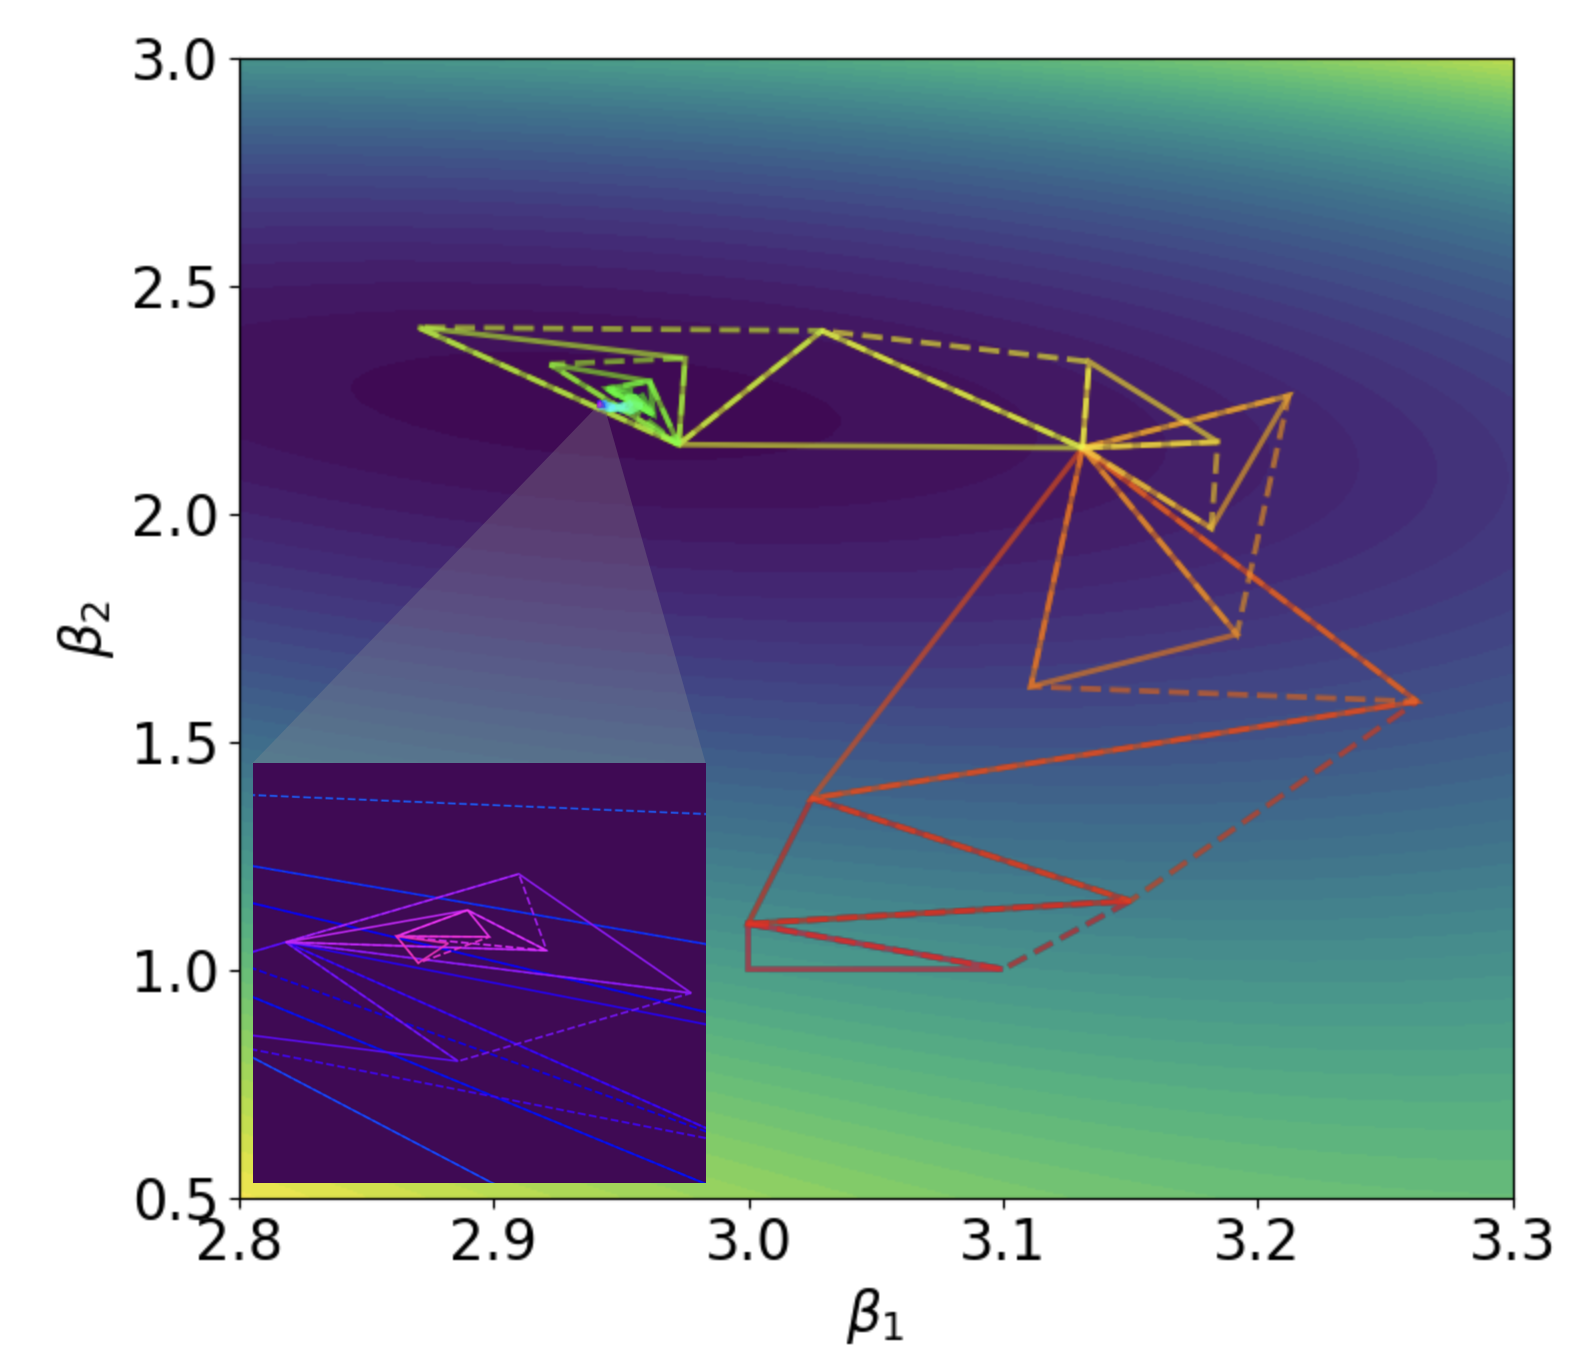
\includegraphics[width=0.6\linewidth]{images/nelder_mead_illustration.png} \caption[Visualising the Nelder-Mead optimisation algorithm.]{Illustration of the Nelder-Mead algorithm for a cost function parameterised by two parameters $\beta_1$ and $\beta_2$. The simplex for a 2-dimensional landscape is a triangle, which then follows the rough algorithm described in the text. The iterations of the algorithm are indicated by constantly switching from solid to dashed edges of the simplex at each step as well as changing in colour. The inset shows a magnification of the final steps of the algorithm.}\label{fig:nelder_mead}
\end{figure}

The way this direct search approach is adapted in Nelder-Mead is by constructing simplices, which are geometric objects that generalise triangles in lower and higher dimensions. For a cost function dependent on $n$ parameters, Nelder-Mead constructs an $n$-dimensional simplex. For $n=0$ this is a point, for $n=1,2,3$ a line segment, triangle and tetrahedron respectively and then higher-dimensional versions as $n$ increases. Thus a simplex has $n+1$ vertices for $n$ parameters. 

The vertices of this simplex then traverse the cost function landscape according to the Nelder-Mead algorithm in order to converge to some minimum value.  In most of the search steps, the primary change is to shift the highest point of the simplex (\@i.e.~where the cost function value is largest) through the opposite face of the simplex, moving to a point with a lower cost function value. These steps are known as \emph{reflections} and they are designed to preserve the volume of the simplex, ensuring it remains non-degenerate. Whenever possible, the method will expand the simplex along a particular direction, which allows it to take bigger steps in search of a minimum. When the simplex encounters a region that can be thought of as a `valley floor' in the cost function landscape, it reduces its dimensions orthogonal to the valley, so that it can slide down. In situations where the simplex has to navigate through a narrow passage, it shrinks itself in all directions, wrapping itself around its best (lowest) point, enabling it to continue its search for the minimum. This process is illustrated for a simple example in Fig.~\ref{fig:nelder_mead}.

This description of the Nelder-Mead method only outlines the basic idea that was first developed in the original 1965 paper. Many variations and improvements have been developed in the years since and the actual implementations. In general, the Nelder-Mead approach is simple to understand and implement, as well as being quite efficient and flexible. However, it often suffers from convergence issues, being both likely to return a sub-optimal local minimum and to get stuck without converging far longer than necessary, undoing any efficiency it otherwise promised. Furthermore, the simplex method doesn't scale well in higher dimensions, making it less effective when the number of parameters is large.

\subsubsection{Powell's method}\label{sec:3.1.3.2_Powell}

Another approach from the gradient-free, local optimiser crowd is Powell's method, first developed by Michael J. D. Powell in 1964 \cite{powell_efficient_1964}. The algorithm is known as a \emph{conjugate-direction} approach, not to be confused with the more common conjugate-gradient approach, although the two are related as the latter can be viewed as a specialisation of the former. 

The basis of Powell's method relies on the idea of conjugate vectors or conjugate directions. Two vectors $\ubb$ and $\boldsymbol{v}$ are said to be conjugate with respect to some positive semi-definite matrix $A$ if $\ubb^T A \boldsymbol{v} = 0$. A set of conjugate directions, thus, is a set of vectors that are pairwise conjugate. Furthermore, one can make the observation \cite{brent_algorithms_2002} that the function
\begin{equation}
    f(\xbb) = \xbb^T A \xbb - 2\boldsymbol{b}^T \xbb + c
\end{equation}
for some positive semidefinite matrix $A$, $\boldsymbol{b} \in \R^n$ and $c \in \R$ has a minimum at the point $\sum_{i=1}^n \beta_i \ubb_i$ in the space spanned by the set of conjugate vectors $\{ u_j \}_{j = 1,...,n}$ with
\begin{equation}
    \beta_i = \frac{\ubb_i^T\boldsymbol{b}}{\ubb_i^T A \ubb_i}.
\end{equation}
This minimum can be calculated efficiently just through evaluating the cost function, without needing explicit access to $A$, $\boldsymbol{b}$ or $c$. This property allowed Powell to develop a simple but powerful gradient-free approach, which can be summarised in the following bit of pseudocode.
\begin{algorithm}
\caption{Powell's Method}
\begin{algorithmic}[1]
\Procedure{Powell}{}
\State Initialise the method with ansatz solution $\ubb_0 \in \R^m$ and $n \leq m$ conjugate search vectors $\{\xbb_1, ..., \xbb_n \}$. If none are provided, use columns of the $m$-dimensional identity matrix.
\For{$i = 1,...,n$}
\State Compute $\beta_i$ to minimise $f(\ubb_{i - 1} + \beta_i \xbb_i)$
\State Define $\ubb_i \gets \ubb_{i - 1} + \beta_i \xbb_i$
\EndFor
\For{$i = 1,...,n-1$}
\State $\xbb_{i} \gets \xbb_{i+1}$
\EndFor
\State $\xbb_n \gets (\ubb_n - \ubb_0)$
\State Compute $\beta$ to minimize $(f(\ubb_0  + \beta \xbb_n))$
\State $\ubb_0 \gets \ubb_0 + \beta \xbb_n$
\EndProcedure
\end{algorithmic}
\end{algorithm}

In other words, the algorithm is initialised with a guess for a solution and a set of conjugate directions. It then proceeds to find a minimum along each direction and shifts to a new point along a superposition of their minima, adding the vector along in which it shifted to the list of conjugate direction vectors and removing the first vector in the list before starting the next step.

\begin{figure}[t]
\centering
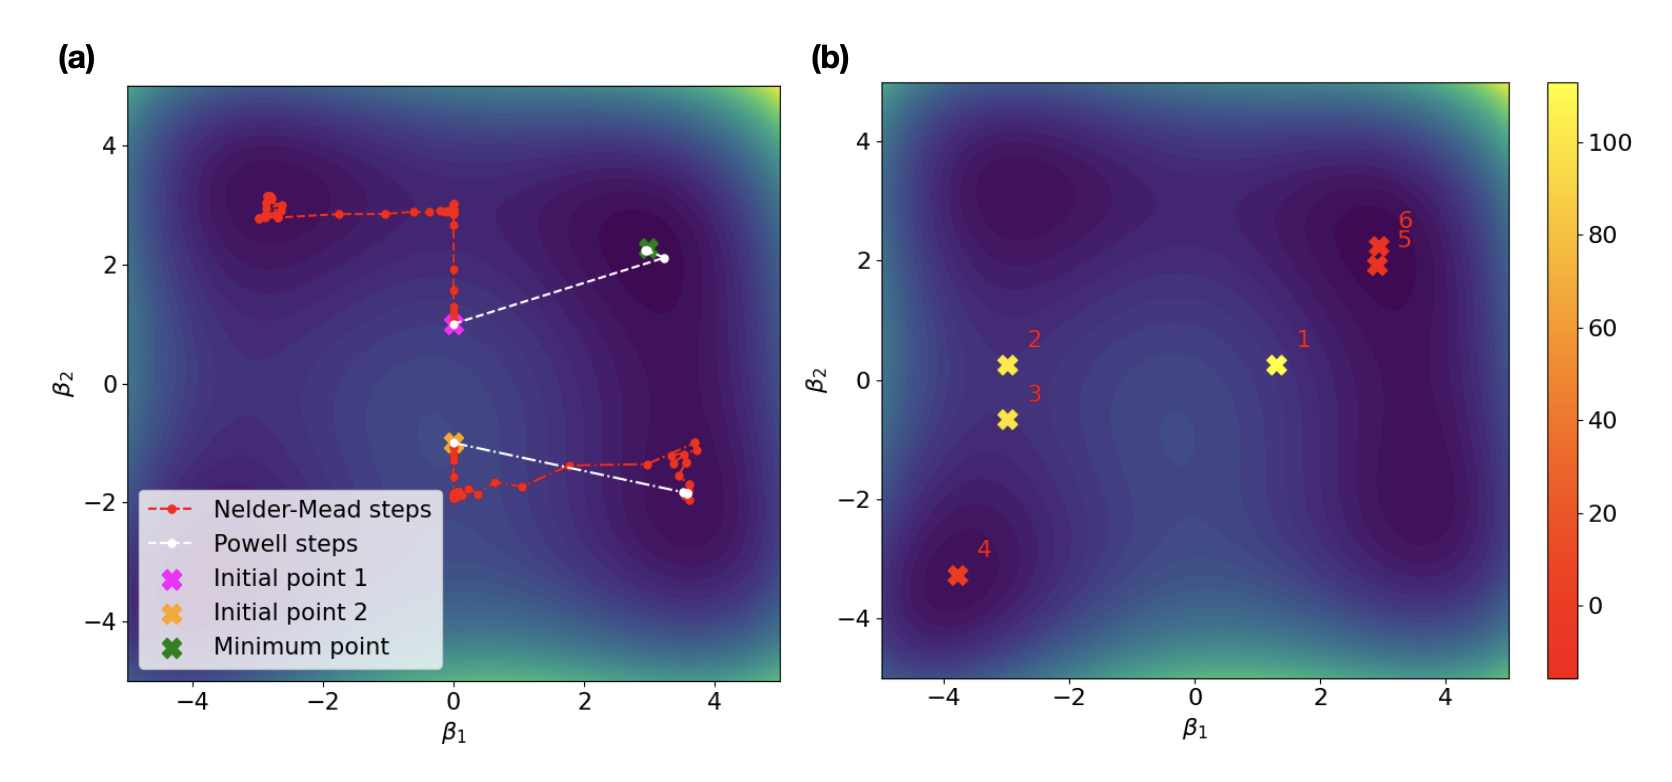
\includegraphics[width=\linewidth]{images/optimiser_plots.png} \caption[Visualising optimisers in action]{An illustration of the optmisation strategy of several numerical optimisation methods. (a) Local optimisers: steps of the Nelder-Mead method and Powell's method when instantiated in two different locations of the loss function landscape. The global mimimum is illustrated by a green cross. (b) The local minima (crosses) visited by the Dual-Annealing in the order indicated by the numbered labels. The colour of the crosses reflects the value of the cost function evaluated at that point as indicated by the colourbar.}\label{fig:optimisers}
\end{figure}

The Powell method is far more complex than is presented here, in particular due to the fact that several extra steps are usually added in order to guarantee convergence and and additional features to help optimise it. Additionally, the minimisation procedure of steps 4 and 11 in the pseudocode is highly non-trivial and can be achieved via several different algorithms like Brent's method\cite{brent_algorithms_2002}. It has guarantees of being very efficient in convex optimisation problems and excels in high-dimensional spaces, unlike Nelder-Mead. A plot of the search steps of the two methods in Fig.~\ref{fig:optimisers}(a) shows how they compare in terms of number of steps taken and accuracy in finding the optimum of some non-convex loss function. Importantly, given the more complicated nature of the steps in Powell's method, the fact that it requires fewer steps to converge to a solution does not necessarily make it more efficient.

\subsubsection{Dual-annealing}\label{sec:3.1.3.3_dual_annealing}

Unlike both Nelder-Mead and Powell's method, dual-annealing is a \emph{global} optimization algorithm, meaning that its primary goal is to find a global minimum of the function. It is also a stochastic method, since rather than follow a pre-defined set of rules or procedures, it employs probabilistic transitions or decisions during the search. This added randomness can help the algorithm escape local optima and explore the solution space more broadly, however it also adds to the computational complexity of such approaches. As mentioned earlier, global optimisation algorithms tend to be far less efficient than local ones, but this is the price that needs to be paid when solutions obtained in local minima are simply not enough and the cost function landscape is highly non-convex. 

What is particularly interesting about dual-annealing is that it combines Generalized Simulated Annealing (\acrref{GSA}) \cite{tsallis_generalized_1996}, a global search algorithm, with a choice of \emph{local} optimiser that refines the solution once the global search is done. This is important because global algorithms, including \acrref{GSA}, are often good at locating the vicinity of the global minimum (the basin) but not necessarily the minimum itself. 

The \acrref{GSA} part of dual-annealing function is, unsurprisingly, a generalisation of the simulated annealing algorithm \cite{kirkpatrick_optimization_1983} inspired by the annealing process of metallurgy which causes a molten metal to reach its crystalline state which is the global minimum in terms of thermodynamic energy. In simulated annealing, the cost function is treated as the energy function of a molten metal and one or more artificial temperatures are introduced and gradually cooled. In \acrref{GSA}, this presents itself as a series of probabilistic jumps across the cost function landscape that depend on an artificial temperature parameter which decreases as the search progresses. 

More concretely, at each step of the search, the algorithm generates a trial jump in the cost function space from the current temporary solution to a new point by sampling it from a modified Cauchy-Lorentz distribution. The distribution peaks around the current temporary solution and its scale parameter (a variable that controls its spread) is a function of the artificial temperature $T_{q_v}$. Thus, the higher the temperature, the more likely it is that the trial jump will be larger. The $q_v$ parameter can be set to different values in order to speed up or slow down the cooling process.

Once the trial jump has been generated, it is either accepted or rejected based on the cost function value at the new point as compared to the current point. If the new point is better (\@i.e.~the jump is `downhill', towards a lower energy), then the jump is accepted. If, on the other hand, the jump is worse or `uphill', it might still be accepted with some probability based on a parameterised Metropolis algorithm \cite{chib_understanding_1995}. This allows for the algorithm to potentially escape local minima. If a jump is accepted, the search then continues in a similar manner from the new point and the temperature parameter is decreased, reducing the probability of the next generated jump being far away from the current point.

The dual-annealing algorithm proceeds by first using \acrref{GSA} to identify a `basin' in the cost function landscape and then using the best solution so far as an initial guess for a local optimisation algorithm like Nelder-Mead or Powell's method to refine the solution. The local search is generally called when the artificial temperature decreases below some pre-defined value and once the local search is done, the whole process restarts again while keeping track of the current best solution. The entire algorithm terminates when some convergence criterion is satisfied. Usually this is when some number of search iterations or cost function evaluations is reached, or there is no more improvement to the solution below some tolerance. This process is illustrated in Fig.~\ref{fig:optimisers}(b), where the dual-annealing algorithm returns points 1, 2 and 4 as minima detected during the annealing stages with 3 and 5 corresponding to minima detected during the local searches. 

The verdict regarding dual-annealing, with respect to the local optimisers that we addressed previously, is that it is far more powerful and can lead to far better solutions, given that it has a far better ability to explore the cost function landscape. However, it is also more computationally expensive, as can be made obvious by the fact that local search is merely a subroutine of the algorithm. Ultimately, the choice of which approach comes down to having knowledge about the cost function landscape as well as trial-and-error. The use of a global optimiser may be overkill when the cost function landscape lends itself well to local methods and each evaluation of the cost function is expensive. If, however, local optimal solutions are not enough, then global methods are by far the best option.

\section{Quantum optimal control}\label{sec:3.2_Quantum_optimal_control}

We've now established that the broad goal of optimal control theory is the design of protocols and strategies which optimise the behaviour of some abstract control system with respect to some abstract target. Quantum optimal control theory (\acrref{QOCT}), rather predictably, does this in the setting where the abstract system is a quantum system. Very broadly then, \acrref{QOCT} concerns itself with the design and analysis of electromagnetic fields that manipulate quantum dynamical processes at the atomic or molecular scale in the best way possible, as illustrated in Fig.~\ref{fig:quantum_optimal_control}. In this chapter, I will broadly cover the basics of \acrref{QOCT}, starting with how the mathematical structure discussed in Sec.~\ref{sec:3.1.1_mathematical_structure} can be adapted to the quantum setting and ending with detailed descriptions of \acrref{CRAB} (Sec.~\ref{sec:3.3.1_CRAB}) and \acrref{GRAPE} (Sec.~\ref{sec:3.3.2_GRAPE}), popular \acrref{QOCT} methods which will be relevant to later work presented in this thesis. As the content of later chapters will focus on closed systems, that will be the perspective I will take with respect to \acrref{QOCT}. More concretely, we will focus on cases where the generator of transformations of a quantum system is primarily modelled as the Hamiltonian as opposed to, \@e.g.~a Liouvillian, but a similar analysis holds in the case of open systems which are just as interesting, if not quite as relevant to this thesis.

Returning to the material covered in Sec.~\ref{sec:3.1.1_mathematical_structure}, we can now add more structure to the abstract notions of system, control function and cost function. In the quantum setting, the set of state functions $X$ often takes the form of a set of quantum states, be they complex vectors, density matrices or operators. The set of control functions $U$ is usually represented by a set of functions of parameterised Hamiltonians. It is common to decompose a control Hamiltonian into two components: the time-dependent `drive' part and the time-independent `drift' part. The time-dependent part can then be further decomposed into a set of $N_k$ operators $\{\mathcal{O}_{\rm opt}^{(k)}\}_{k=1,...,N_k}$, such that the full control Hamiltonian reads:
\begin{equation}\label{eq:optimal_control_H}
    H(\ubb(t)) = H_0 + \sum_{k = 1}^{N_k} u_k(t) \mathcal{O}_{\rm opt}^{(k)},
\end{equation}
where $H_0$ is the drift Hamiltonian with no external controls and the control functions $u_k(t) \in \ubb(t)$ drive the corresponding operators $\mathcal{O}_{\rm opt}^{(k)}$.

\begin{figure}[t]
\centering
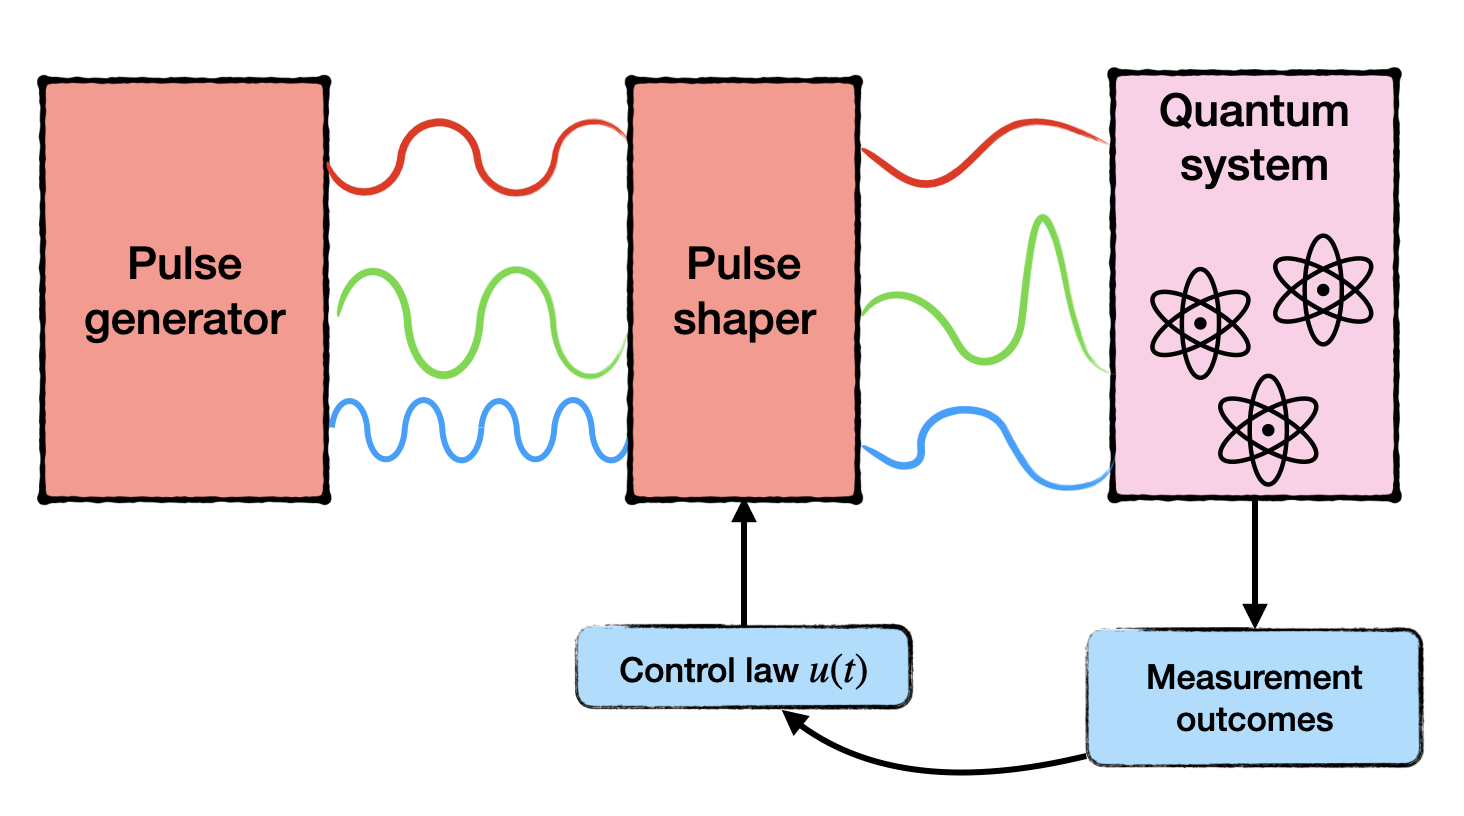
\includegraphics[width=0.8\linewidth]{images/optimal_control_placeholder.png} \caption[Schematic diagram of open-loop quantum optimal control]{A sketch of a quantum optimal control closed-loop set-up. A quantum system is directly controlled by a set of electromagnetic pulses which are shaped according to a set of control functions $\ubb(t)$ that are optimised based on feedback from the information obtained through measurements of the system.}\label{fig:quantum_optimal_control}
\end{figure}

Given this, we can describe a general quantum optimal control problem in analogy to Eq.~\eqref{eq:control_ODE} as one where the aim is to solve the Schr\"{o}dinger equation:
\begin{equation}\label{eq:optimal_control_schroedinger}
    i \hbar \partial_t \ket{\psi(t)} = H(\ubb(t))\ket{\psi(t)},
\end{equation}
with the constraint of starting in a state from a set of initial states $\ket{\psi_0} \in \boldsymbol \Psi_0$ and while minimising some cost function that targets a set of final states $\ket{\psi_T} \in \boldsymbol \Psi_T$. I should note that while I am using wavefunctions as representations for the states of the control system, it is actually quite common in \acrref{QOCT} to instead work in the operator picture, where the Schr\"{o}dinger equation is
\begin{equation}\label{eq:operator_schroedinger_eq}
    \partial_t \mathcal{O}(t) = -i H(\ubb(t))\mathcal{O}(t),
\end{equation}
where $\mathcal{O}$ is an operator on some pre-defined Hilbert space. A useful constraint in this setting is to take the initial state of the operator to be the identity $\mathcal{O}(0) = \mathds{1}$. The choice of wave mechanics or matrix mechanics depends on the specific \acrref{QOCT} problem at hand, although questions of \@e.g.~ controllability are usually best-solved with operators rather than state vectors. For example, if we can show that the set of possible matrices that can be obtained for system \eqref{eq:operator_schroedinger_eq} is the set of all the unitary matrices (with the rank of the system Hilbert space), then the system can theoretically be steered to any arbitrary state and thus it is controllable.

The choice of cost function in the quantum setting is generally informed by the desired properties of the target state(s) combined with considerations for what information can be extracted from the system and other constraints. For example, when the aim of the optimisation is to prepare a single, well-defined quantum state $\ket{\psi_T}$ with high accuracy, then the most informative cost function is:
\begin{equation}\label{eq:costfunc_fidelity}
    C_F(\tau, \ubb) = 1 - F(\tau, \ubb) = 1 - \abs{\braket{\psi(\tau, \ubb)}{\psi_T}}^2,
\end{equation}
where $F(\tau, \ubb)$ is the fidelity of the final state $\ket{\psi(\tau, \ubb)}$ with respect to the desired target $\ket{\psi_T}$. Here $\ket{\psi(\tau, \ubb)}$ is generated by driving an initial state $\ket{\psi_0} \in \boldsymbol \Psi_0$ for a time $\tau$ via the time-dependent Hamiltonian $H(\ubb(t))$. If, on the other hand, the target state need only be a ground state of some Hamiltonian $H_T$, then it might be far more convenient to use the final system energy:
\begin{equation}\label{eq:costfunc_energy}
    C_E(\tau, \ubb) = \mel{\psi(\tau, \ubb)}{H_T}{\psi(\tau, \ubb)}.
\end{equation}
Finally, should one be interested only in a specific property of the final state, like its entanglement, then the cost function might look something like:
\begin{equation}\label{eq:costfunc_entanglement}
    C_S(\tau, \ubb) = -S[\ket{\psi(\tau, \ubb)}],
\end{equation}
where $S[\cdot]$ is some appropriate measure of entanglement. As well as being informed by the set of target states, the cost function may include further constraints, like the total power of the driving fields in the Hamiltonian. This is analogous to the cost function in Eq.~\eqref{eq:example_cost_func2}, which in the quantum case might look something like:
\begin{equation}\label{eq:costfunc_constraint}
    C(\tau, \ubb) = C_F(\tau, \ubb) + \sum_{k = 1}^{N_k} \int_0^{\tau} \abs{u_k(t)}^2 dt,
\end{equation}
which can be read as an optimisation for final state fidelity with the added constraint that the time-integrated flux of the driving fields is minimised. 

\section{Quantum optimal control methods}\label{sec:3.3_qoct_methods}

Both analytical (Sec.~\ref{sec:3.1.2_analytic_optimisation}) and numerical (Sec.~\ref{sec:3.1.3_numerical_optimisation}) methods have been developed for the optimal control of quantum systems in recent decades. Analytical methods in \acrref{QOCT} generally deal with questions of necessary conditions for controllability \cite{schirmer_complete_2001} or reachability of states, \@e.g.~exploring quantum speed limits \cite{khaneja_time_2001, hegerfeldt_driving_2013, poggi_quantum_2013}. Analytical methods \emph{can} be used to find solutions to quantum optimal control problems rather than just classify their structure, but the Achilles' heel of analytical approaches remains a general inability to deal with complex systems. The volatile and often exponentially complex nature of quantum systems means that numerical approaches tend to be the preferred method for actually determining solutions to \acrref{QOCT} problems. 

Numerical methods in \acrref{QOCT} tend to consist of the development and analysis of iterative algorithms focused on optimising pulses for quantum systems. This can be done by constructing a mathematical description of the pulse, including parameters that control its shape and which can then be numerically optimised. Most numerical methods under the umbrella of \acrref{QOCT} involve a classical optimiser, like those discussed in Sec.~\ref{sec:3.1.3_numerical_optimisation}, as a subroutine in the approach which finds the optimal values for the pulse parameters. In this section I will explore two of the more broadly used numerical approaches in quantum optimal control, \acrref{CRAB} and \acrref{GRAPE}. 

\subsection{Chopped random-basis quantum optimization (CRAB)}\label{sec:3.3.1_CRAB}

The ``Chopped random-basis quantum optimization" or \acrref{CRAB} method is a quantum optimal control method first introduced in \cite{doria_optimal_2011, caneva_chopped_2011} which revolves around the construction of a truncated randomized basis of functions for the control fields of a quantum system. It was originally developed for quantum many-body systems whose time evolution can be efficiently simulated by time-dependent density matrix renormalization group (tDMRG)\cite{white_density_1992, schollwock_density-matrix_2005, schollwock_density-matrix_2011}. It was believed that such systems were mostly intractable for control optimization using gradient-based algorithms \cite{brif_control_2010}, although such potential limitations have been overcome in more recent work\cite{jensen_approximate_2021}. \acrref{CRAB} provides a way to reduce the space of search parameters, making the optimisation process more efficient, while retaining access to a large solution space through the added randomisation component.

The key idea is to expand the control pulse $\ubb(t)$ in some truncated basis of dimension $N_k$: 
\begin{equation}\label{eq:basic_CRAB}
    u(t) = \sum_{i = 1}^{N_k} c_i u_i(t),
\end{equation}
where the cost function landscape is spanned by the coefficients $c_i$, that need to be optimised over using numerical optimisation methods like those described in Sec.~\ref{sec:3.1.3_numerical_optimisation}. Generally this basis is made up of trigonometric functions although it could be any basis that spans the space of admissible controls \@e.g.~generalized Chebyshev polynomials. A choice of basis can further be enhanced or modified by a shape function $g(t)$ that fixes the pulse to some initial and/or final value:
\begin{equation}\label{eq:trigonometric_CRAB}
    u(g(t),t) = \sum_{i = 1}^{N_k/2} c_i \frac{\cos{\omega_i t}}{g(t)} + \sum_{i = N_k/2 + 1}^{N_k} c_i \frac{\sin{\omega_i} t}{g(t)}.
\end{equation}

Importantly, the key to expanding the solution space in order to find better pulses using the \acrref{CRAB} approach lies in the randomisation of the frequencies $\omega_i$. During each optimisation process, the $\omega_i$ are chosen randomly around the principal harmonics within some interval $[0, \omega_{\rm max}]$, allowing the pulse shapes to be more diverse and more complex than by simply keeping them fixed at a certain value. The optimisation process can then be parallelised, with several optimisation instances running simultaneously exploring several different sets of random frequencies and the optimal solution can be picked from the final outcomes of all optimisations. 

The \acrref{CRAB} approach lends itself very easily to the incorporation of additional features and constraints like the shape function. For example, it is quite easy to start with a trial pulse, say $f(t)$, which cannot be expanded efficiently or exactly in the chosen basis and to dress it according to
\begin{equation}\label{eq:trial_pulse_CRAB}
    u(t) = f(t)\Bigg(1 + \sum_{i = 1}^{N_k} c_i u_i(t)\Bigg).
\end{equation}
Another particularly useful alteration to the basic \acrref{CRAB} procedure is what is known as `dressed' \acrref{CRAB} or dCRAB \cite{rach_dressing_2015}, which in a similar vein aims to iteratively re-dress solutions obtained from previous optimisations with new sets of basis functions added onto the existing solution. These \emph{super-iterations} $j$ can be modelled as
\begin{equation}\label{eq:dCRAB}
    u^j(t) = c_0^j u^{j-1}(t) + \sum_{i = 1}^{N_k} c_i^j u^j_i(t)
\end{equation}
where $u^j_i(t)$ are new basis functions and $u^{j-1}(t)$ is the pulse obtained from a previous, $(j-1)^{\rm st}$ optimisation. The coefficient $c_0^j$ can be seen as shifting the solution in the direction of the previous solution pulse while $\{ c_i^j\}_{i = 1, ..., N_k}$ move it in new search directions $u^j_i(t)$. This is, in fact, very similar to Powell's optimisation method which I covered in Sec.~\ref{sec:3.1.3.2_Powell}, wherein a finite set of search directions in cost function space is continuously updated with linear combinations of their optima. dCRAB can be seen as doing the same but with updates sampled from an infinite-dimensional search space. This iterative approach is useful in  avoiding local minima and in exploring a far larger search space, avoiding the hard constraint of a finite set of basis functions for each optimisation. 

There are several key advantages in the \acrref{CRAB} approach that have led to its widespread use in the \acrref{QOCT} community. For one, the randomization of the control field basis allows for a more comprehensive exploration of the control landscape, which can lead to the discovery of better solutions. It also offers relatively quick convergence as the number of optimisable parameters is usually small when compared to other approaches (such as \acrref{GRAPE}, which we will explore in the next section). Finally, it is very flexible: the basis functions can be altered and constraints can be incorporated quite easily, whether they concern the physical implementation (\@e.g.~the shaping function) or some efficiency concerns (à la dCRAB).

\subsection{Gradient Ascent Pulse Engineering (GRAPE)}\label{sec:3.3.2_GRAPE}

The ``Gradient Ascent Pulse Engineering" (GRAPE) algorithm is yet another widely used \acrref{QOCT} numerical method. It was first developed in order to design pulse sequences in NMR spectroscopy \cite{khaneja_optimal_2005} and has since been iterated upon and improved a number of times as well as being integrated into several optimal control packages \cite{de_fouquieres_second_2011, chen_iterative_2022, machnes_comparing_2011, johansson_qutip_2013}. As the name suggests, it is a gradient-based optimisation method and while initially it was used primarily for the preparation of specific target states, its powerful flexubility has since lent itself to many other applications in the setting of quantum technologies, like the optimisation of quantum logic gates \cite{motzoi_optimal_2011, anderson_accurate_2015}.

The key idea behind \acrref{GRAPE} is to replace continuous control functions, like \@e.g.~those used in the basis functions of \acrref{CRAB}, with piecewise constant control amplitudes $u_j(t_k)$, each applied to the control system at time $t_k \in [0, \tau]$ for a time interval $\Delta t$, where $\tau$ is the total evolution time. You can view this as discretizing the time-evolution of the system into $N_m$ slices of time $\Delta t = t_{k + 1} - t_k$. These slices need not all be of equal size, but for simplicity let us work in the setting where they are, meaning that $\tau = N_m \Delta t$.

At this point we can pause and notice that since the control amplitudes $u_j(t_k)$ are piecewise constant for all time intervals, they can be treated as a set of parameters that can be optimised using a numerical optimisation algorithm. This gives $N_j \cross N_m$ total parameters to optimise, as each $j^{\rm th}$ pulse will be made up of $N_m$ time-steps. Given this relatively large number of parameters, the original \acrref{GRAPE} algorithm included an analysis of how to compute the gradient of the cost function with respect to each $u_j(t_k)$ in order to implement gradient-based optimisation methods like gradient-descent (Eq.~\eqref{eq:gradient_descent}). Recalling the form of the quantum control Hamiltonian from Eq.~\eqref{eq:optimal_control_H}, the propagator for the time-evolution of the quantum system using \acrref{GRAPE} during a single time step $\Delta t$ at time $t_k$ is
\begin{equation}
    U_k(\Delta t) = \exp{- i \Delta t \Big( H_0 + \sum_{j=1}^{N_j} u_j(t_k) \mathcal{O}_{\rm opt}^{(j)} \Big)}
\end{equation}
for some drift component of the Hamiltonian $H_0$ and some basis of control operators $\{\mathcal{O}_{\rm opt}^{(j)}\}_{j = 1,...,N_j}$. The full evolution of the system can thus be captured by the product of operators (with dependence on $\Delta t$ removed):
\begin{equation}
    U(\tau) = U_{N_m} U_{N_m - 1} ... U_{2} U_{1},
\end{equation}
such that for some initial state $\rho_0$ (where we are now working with density matrices rather than state vectors), the final evolved state can be written as
\begin{equation}\label{eq:grape_rho_evolved}
    \begin{aligned}
        \rho(\tau) &= U(\tau)\rho_0 \adj{U}(\tau) \\
        &= U_{N_m} ... U_{1} \rho_0 \adj{U}_{1} ... \adj{U}_{N_m}
    \end{aligned}
\end{equation}

At this point, in order to derive a way to compute the gradient of the cost function with respect to the parameters, it is necessary to define a cost function. In this case we will use the overlap of the final state $\rho(\tau)$ with respect to some target state $\rho_T$, a density matrix version of Eq.~\ref{eq:costfunc_fidelity}:
\begin{equation}
    C(\ubb) = \Tr{\rho_T^{\dagger}\rho(\tau)},
\end{equation}
where $\ubb$ in this case is the set of all $N_j \cross N_m$ parameters to be optimised $\ubb: \{ u_j(t_k)\}_{j = 1, ..., N_j}^{k = 1,...,N_m}$. Using Eq.~\ref{eq:grape_rho_evolved} and the cyclic property of the trace we can write
\begin{equation}\label{eq:grape_costfunc_rewrite}
    \begin{aligned}
        C(\ubb ) &= \Tr{\rho_T^{\dagger}U_{N_m} ... U_{1} \rho_0 \adj{U}_{1} ... \adj{U}_{N_m}} \\
        &=  \Tr{\adj{U}_{k+1} ... \adj{U}_{N_m} \rho_T U_{N_m} ... _{k+1} U_{k} ... U_{1} \rho_0 \adj{U}_{1} ... \adj{U}_{j}} \\
        &= \Tr{\Lambda_k \rho_k},
    \end{aligned}
\end{equation}
where $\Lambda_k = \adj{U}_{k+1} ... \adj{U}_{N_m} \rho_T U_{N_m} ... _{k+1}$ and $\rho_k = U_{k} ... U_{1} \rho_0 \adj{U}_{1} ... \adj{U}_{j}$. 

In order to calculate the gradient of $C(\ubb)$ with respect to each parameter $u_j(t_k)$, we first investigate what happens to $U_k$ when we perturb each parameter by some small amount $\delta u_j(t_k)$. To first order in $\delta u_j(t_k)$ we get
\begin{equation}
    \delta U_k = -i \delta u_j(t_k) U_k \int_0^{\Delta t} U_k(t') \mathcal{O}_{\rm opt}^{(j)} U_k(-t') dt'.
\end{equation}
Then, for small $\Delta t$ (\@i.e.~when it is much smaller than the norm of the control Hamiltonian), we find that the integral in the expression above can be approximated as the average value of the integrand, leading to:
\begin{equation}\label{eq:grape_costfunc_gradient}
    \frac{\delta C(\ubb)}{\delta u_j(t_k)} = - \Tr{\Lambda_k \Big(i\Delta t \comm{\mathcal{O}_{\rm opt}^{(j)}}{\rho_k}\Big)}.
\end{equation}

Using this, it is now possible to implement gradient-based numerical optimisation algorithms in order to find optimal values of $\ubb$, in the vein of gradient-descent from Eq.~\ref{eq:gradient_descent}. The method has been improved upon after the initial algorithm was first published, \@e.g.~in \cite{machnes_comparing_2011} in order to include information about second-derivatives of the cost function, allowing for more complex gradient-based optimisation like quasi-Newton methods (see discussion in Sec.~\ref{sec:3.1.3_numerical_optimisation}). Recent years have also seen improvements similar to those of dCRAB in the case of the \acrref{CRAB} algorithm, where an iterative optimisation procedure is applied on top of the basic \acrref{GRAPE} algorithm \cite{chen_iterative_2022}. It would be pertinent to mention, that there are very similar approaches to constructing \acrref{GRAPE}-type pulses out in the literature known as Krotov schemes \cite{reich_monotonically_2012}. The key difference between \acrref{GRAPE} and Krotov is in the update step in the iterative optimisation procedure: where the \acrref{GRAPE} algorithm updates all control parameters in a single iteration at once, the Krotov-based methods do so sequentially. Furthermore, Krotov-based approaches are only well-defined in the continuum limit \@i.e.~where the time step $\Delta t \ll 1$, which need not be the case for many implementations of \acrref{GRAPE}. In fact, Krotov approaches have been shown to be monotonically convergent in that limit \cite{morzhin_krotov_2019}, so they can suffer in the face of discretisation, something that is a roadblock for some implementations. \acrref{GRAPE} escapes this fate and, despite in many ways being less sophisticated, can be far more efficient in more restrictive settings with large time steps far away from the continuum limit.

Ultimately, \acrref{GRAPE} is a simple and powerful approach to constructing a control pulse, but it can suffer from the large number of parameters that need to be optimised. In more simple settings, where the cost function is smooth and convex, it is a very powerful tool, as on top of the high degree of control over the exact shape of the pulse, it offers a gradient-based method level of convergence. Gradient-based methods, as discussed in Sec.~\ref{sec:3.1.3_numerical_optimisation}), are efficient and converge rapidly given convexity guarantees, regardless of the number of parameters that describe the control function. There has been a lot of work done in recent years analyzing the topological and mathematical properties of quantum control landscapes, including their smoothness \cite{chakrabarti_quantum_2007, rabitz_surprising_2023,dong_quantum_2022}, although these only apply to problems where the cost function is ``well behaved" - \@i.e.~is some polynomial of the final state vector or matrix which itself evolves continuously on a smooth manifold.  However, there is no reason to expect that the cost function landscape will be particularly smooth nor convex in any specific instance, meaning the gradient information obtained in the \acrref{GRAPE} algorithm may not be useful. Furthermore, the gradient evaluation step can be quite computationally intensive. At the end of the day, one can always construct a \acrref{GRAPE}-type pulse and optimise the many parameters using, for example, a global optimiser like dual-annealing from Sec.~\ref{sec:3.1.3.3_dual_annealing}, but given how high-dimensional the problem might be due to the many parameters involved, this can be a very computationally intensive task.

It is useful to compare \acrref{GRAPE} and \acrref{CRAB}, as each offers a different set of advantages and disadvantages. The effectiveness of \acrref{CRAB}, for example, relies a lot on the choice of basis functions used in constructing the pulse, but the number of parameters to be optimised is generally far lower than that of \acrref{GRAPE}. Both offer a lot of flexibility in terms of incorporating constraints and using different numerical optimisers, although \acrref{CRAB} generally does not include a systematic way to compute cost function gradients, leaving it subject to gradient-free methods. 
\part{Counterdiabatic optimised local driving}

\chapter{The \acrref{COLD} method}\label{chap:4_COLD}

Having now covered both \acrref{CD} and optimal control, we can proceed to the main result I want to explore in this thesis: that of 

\section{The recipe}

\begin{equation}\label{eq:expandedH}
H_{\rm COLD}(\lambda,\betabb) = H_0(\lambda) + {\boldsymbol \alpha}(\lambda,\betabb) \mathcal{O}_{\rm LCD} + \betabb(\lambda) \mathcal{O}_{\rm opt}.
\end{equation}

\section{Higher-order \acrref{CD} as a cost function}

\begin{equation}\label{eq:AGP_integral_1}
\mathcal{I}_1 = \int_0^\tau dt^\prime \Big[\bra{\psi_g(t^\prime)} \Gamma^2(t^\prime) \ket{\psi_g(t^\prime)}  - (\bra{\psi_g(t^\prime)} \Gamma(t^\prime) \ket{\psi_g(t^\prime)})^2\Big]^{1/2},
\end{equation}

\begin{equation}\label{eq:Gamma_def}
\Gamma(t) = \gamma(t) \left( \sy_1 \sx_2 + \sx_1 \sy_2 \right),
\end{equation}

\begin{equation}\label{eq:AGP_integral_2}
\mathcal{I}_2 = \int_0^\tau dt^\prime |\gamma(t^\prime)|,
\end{equation}
\chapter{Adiabatic gauge potential as a cost function}\label{chap:5_cd_as_costfunc}

\epigraph{Always remember, however, that there’s usually a simpler and better way to do something than the first way that pops into your head.}{\emph{Donald Knuth}}

In the previous chapter I presented the counterdiabatic optimised local driving or \acrref{COLD} method, which combines \acrref{LCD} (Sec.~\ref{sec:2.4.1_LCD}) and quantum optimal control (Sec.~\ref{sec:3.2_Quantum_optimal_control}) in order to speed up adiabatic quantum processes while minimising transitions out of the instantaneous eigenstates. The strategy of \acrref{COLD} is largely concerned with implementing optimal control in order to modify the path of the time-dependent Hamiltonian in parameter space in a way that maximises the effectiveness of a given \acrref{LCD} drive in driving a system to a target eigenstate of the adiabatic Hamiltonian. The optimal control component of \acrref{COLD} is thus constructed around optimising for the final state of the system after evolution: whether by assessing its fidelity with respect to some target state or a property like entanglement.

In this chapter we will take a slightly different but complementary perspective on combining \acrref{LCD} and optimal control by asking the question of what happens when, instead of optimising for a particular target state, we use only information about the counterdiabatic drive - or rather, the adiabatic gauge potential (\acrref{AGP}) from Sec.~\ref{sec:2.2_AGP} - as the optimal control cost function. Since the \acrref{AGP} contains information about the non-adiabatic effects experienced by a system, it is reasonable to believe that this information can be extracted and its analysis can be useful in designing optimal fast driving schedules for adiabatic protocols. 

I will begin the chapter with a brief motivation behind using the counterdiabatic pulse as a metric for optimising fast adiabatic processes in Sec.~\ref{sec:5.1_motivation} and then in Sec.~\ref{sec:5.2_designing_costfunc_hocd} we will explore several different ways in which the \acrref{CD} pulse can be transformed into an optimal control cost function. While this chapter will introduce the theory behind the idea, Ch.~\ref{chap:7_higher_order_agp} will present the numerical simulation results obtained using the ideas in this chapter.

\section{Motivation}\label{sec:5.1_motivation}

Returning to the key ideas behind \acrref{CD}, we may recall that the exact \acrref{CD} pulse is comprised of the \acrref{AGP} (Sec.~\ref{sec:2.2_AGP}) operator $\AGP{\lambda}$ scaled by the rate of change of $\lambda(t)$ (expressed as $\dotlambda$) in the adiabatic Hamiltonian, as given by Eq.~\eqref{eq:CD_Hamiltonian}. The \acrref{AGP} is the generator of adiabatic deformations between quantum eigenstates, and its off-diagonal elements are responsible for transitions between the instantaneous (or adiabatic) eigenstates or, put another way, the Frobenius norm of the \acrref{AGP} is the distance between nearby eigenstates \cite{pandey_adiabatic_2020, nandy_delayed_2022} \textcolor{red}{@ Callum this is correct, I've changed the references to where this exact thing is stated exactly like this (and I have more) and described in detail. Is it the wording that's confusing somehow?}. Thus, there are two components comprising the non-adiabatic effects experienced by a system driven at finite time by a time-dependent Hamiltonian: the rate of change of the parameters $\dotlambda$ and the \acrref{AGP} operator, which can be quantified \@e.g.~via its norm. 

In the design fast adiabatic protocols such as the techniques under the umbrella of \acrref{STA}, we are competing against $\dotlambda$ as the aim in general is speed rather than adherence to the adiabatic condition. This leaves us with minimising $\AGP{\lambda}$ or else, as in the case of \acrref{CD}, suppressing or mitigating its effects. To whit, \acrref{LCD} does this by implementing an operator that approximately suppresses the \acrref{AGP} for a given Hamiltonian. \acrref{COLD} then aids in this endeavour by modifying the Hamiltonian and thus the corresponding \acrref{AGP} operator in a way that allows for a given \acrref{LCD} protocol to perform better. The optimal control component of \acrref{COLD} in \cite{cepaite_cold_2023} and throughout Ch.~\ref{chap:6_Applications_fidelity} is implemented with the target state fidelity (Eq.~\eqref{eq:costfunc_fidelity}) as a cost function, which is down to the fact that the primary application of adiabatic protocols in often (though not always \cite{pelegri_high-fidelity_2022}) state preparation. The use of fidelity as a cost function, however, necessitates access to the wavefunction of the final state, something that becomes difficult to compute for large or highly correlated systems and may result in a highly non-convex or complex cost function landscape (see, for example, Fig.~\ref{fig:ghz_contours}). Furthermore, fidelity is not a useful cost function in practice in the case where the target state is unknown, which is common in \@e.g.~applications of adiabatic protocols to Hamiltonians whose ground states encode solutions to combinatorics problems \cite{ebadi_quantum_2022, albash_adiabatic_2018}. 

A solution to the problem of fidelity as a cost function might be the use of a different metric for optimising the Hamiltonian path. We have established that $\AGP{\lambda}$ contains information pertaining to non-adiabatic losses experienced by a driven system, thus a natural approach to optimising the path of the Hamiltonian would be to minimise the \acrref{AGP} operator (I will discuss the details of this in the next section), as this should in principle minimise losses associated with non-adiabaticity. The main advantages of such an approach would be the fact that  the minimisation should be far more efficient than any attempt to compute the full system evolution, assuming we have access to the \acrref{AGP} as a function of the Hamiltonian path in parameter space. Furthermore, this process would require no knowledge of the system wavefunction at any point, removing the drawbacks discussed earlier concerning the fidelity cost function.

\section{Designing a cost function around the counterdiabatic pulse}\label{sec:5.2_designing_costfunc_hocd}

There are several ways to define a metric on a time-dependent pulse and in this thesis we will explore two in particular. In order to do this, we will first return to Ch.~\ref{chap:4_COLD}, where we expressed the \acrref{CD} pulse as a sum of operators $\{\mathcal{O}_{\rm CD}^{(j)}\}_{j = 1, ..., N_{\rm CD}}$ which are scaled by coefficients $\alpha_j(\lambda, \hbb)$ with $\lambda$ a function of time and $\hbb$ the $\lambda$-dependent coefficients of the Hamiltonian $H(\lambda)$. In the \acrref{LCD} case, this sum is truncated to a set of operators $\{\mathcal{O}_{\rm LCD}\} \subset \{\mathcal{O}_{\rm CD}\}$ which are themselves scaled by a different set of coefficients $\alpha_j^{\prime}(\lambda, \hbb)$. Expressed this way, we can view the operators as static, with the $\lambda$- and $\hbb$-dependent coefficients $\alpha_j$ and $\alpha_j^{\prime}$ encoding the shape of the pulse and containing the information about non-adiabatic effects for given values of $\lambda$ and $\hbb$. If we include an optimal control component parameterised by functions $\beta_k(\lambda) \in \betabb$ as in Eq.~\eqref{eq:COLD_optimal_control} in the case of \acrref{COLD}, then the counterdiabatic coefficients become dependent on $\betabb$ too, allowing us to optimise them by varying the control functions.

Given this form for the counterdiabatic pulses, we can choose two types of metrics: one which looks at the whole pulse, whether in the case of the exact \acrref{AGP} or some truncation obtained using \acrref{LCD} and another which instead only picks out an extremum of the pulse, like its maximum amplitude. In the first case, a natural option would be the time-integrated absolute value of the $\alpha_j$ coefficients, which in the optimal control community is often referred to as the ``control effort"\cite{petersen_control_1987}:
\begin{equation}\label{eq:COLD_costfunc_integral}
    C_I(\tau, \betabb) = \sum_j^{N_I} \int_{0}^{\tau} dt^{\prime} |\alpha_j^{\prime}(\lambda(t^{\prime}), \hbb, \betabb)|,
\end{equation}
where, as before, $\tau$ is the total driving time and here we take the sum over $N_I$ coefficients. When the quantity $C_I(\tau, \betabb)$ is minimised, naturally the contribution of the operators scaled by the coefficients in the sum will be reduced. When it is $0$, then these operators will not contribute at all to the non-adiabatic losses experienced by the driven system. It should be noted that understanding the physical meaning behind non-zero values of $C_I$ is quite non-trivial, although it is natural to expect that the larger it is, the more losses the system experiences. 

In the case where we want to minimise the exact \acrref{AGP}, $N_I = N_{CD}$. On the other hand, when it comes to \acrref{LCD} it may be fruitful to minimise $\alpha_j^{\prime}$ corresponding to operators which are not actually applied to the system. What this means is that should one have access to a set of operators that have a non-zero contribution to the exact \acrref{CD}, \@e.g.~via the nested commutator approach from Sec.~\ref{sec:2.4.2_nested_commutators}, but it is only possible to physically implement a subset of these, then it is sensible to optimise for a path which minimises the contribution of the subset of operators that cannot be implemented, as this should theoretically reduce their contribution to the non-adiabatic losses. In this way, an \acrref{LCD} protocol can be used to both suppress non-adiabatic losses by the application of an approximate counterdiabatic drive and in order to optimise for a Hamiltonian path which reduces the non-suppressed losses experienced by the system.

The second option for a cost function which uses nothing but the counterdiabatic pulse coefficients is one which instead minimises some extremum of the entire pulse, such as the maximal absolute amplitude reached by the pulse throughout the evolution, which we will write as:
\begin{equation}\label{eq:COLD_costfunc_maximum}
    C_A(\tau, \betabb) = \max_{t^{\prime} \in [0,\tau]} \left( \sum_j^{N_I} | \alpha_j(\lambda(t^{\prime}), \hbb, \betabb)|\right).
\end{equation}

Intuitively, if the integral cost function is $0$, then this second approach does not provide any more information as the two will be equivalent. However, what this cost function captures is whether or not the path of the system for a given $\betabb$ and $\tau$ experiences any critical point in its evolution where the non-adiabatic effects are maximised, for example in the case of closing gaps between the instantaneous eigenstates. This cost function may be useful in cases where one wants to avoid such closing gaps within the system evolution and no path optimally suppresses all non-adiabatic effects. In particular, it might be used in \acrref{LCD} as a means to avoid cases where the \acrref{CD} operators which are not applied are responsible for most of the avoided transitions out of the instanteous eigenstate.
\part{Applications of COLD}

\chapter{Optimising for properties of the state}\label{chap:6_Applications_fidelity}

The previous chapter established the \acrref{COLD} approach, a new method for speeding up adiabatic dynamics which combines local counterdiabatic driving (\acrref{LCD}), discussed in detail in Sec.~\ref{sec:2.4.1_LCD} and  

\section{Two-spin annealing}\label{sec:5.1_2spin_annealing}

One of the simplest example systems to illustrate the \acrref{COLD} method is that of a two-spin model and a simple annealing protocol:
\begin{equation}\label{eq:two_spin_hamiltonian}
H_0(\lambda) = -2J \sz_1 \sz_2 - h ( \sz_{1} + \sz_{2}) +  2h \lambda (\sx_{1} + \sx_{2}),
\end{equation}
where the Hamiltonian is parameterised by the set of coefficients $\{J, h, \lambda(t)\}$, with the $\lambda$ term encoding the time-dependence. For this example we use
\begin{equation}\label{eq:lambda_func1}
\lambda(t) = \sin^2\left(\frac{\pi}{2} \sin^2 \left( \frac{\pi t}{2 \tau} \right) \right),
\end{equation}
such that $\lambda(0) = 0$ and $\lambda(\tau) = 1$. In this way, the transverse field is tuned from $0$ to $2h$ as $t$ goes from $0$ to $\tau$.

\begin{equation}\label{eq:two_spin_alpha}
\alpha = - \frac{h^2}{4(h\lambda)^2 + h^2 + 4J^2}.
\end{equation}

\begin{equation}\label{eq:H_optimal_control}
H_\beta(\lambda) = H_0(\lambda) + \sum_{k=1}^{N_k} \beta^k \sin (\pi k \lambda) ( \sz_{1} + \sz_{2}),
\end{equation}

\begin{figure}[t]
    \centering
    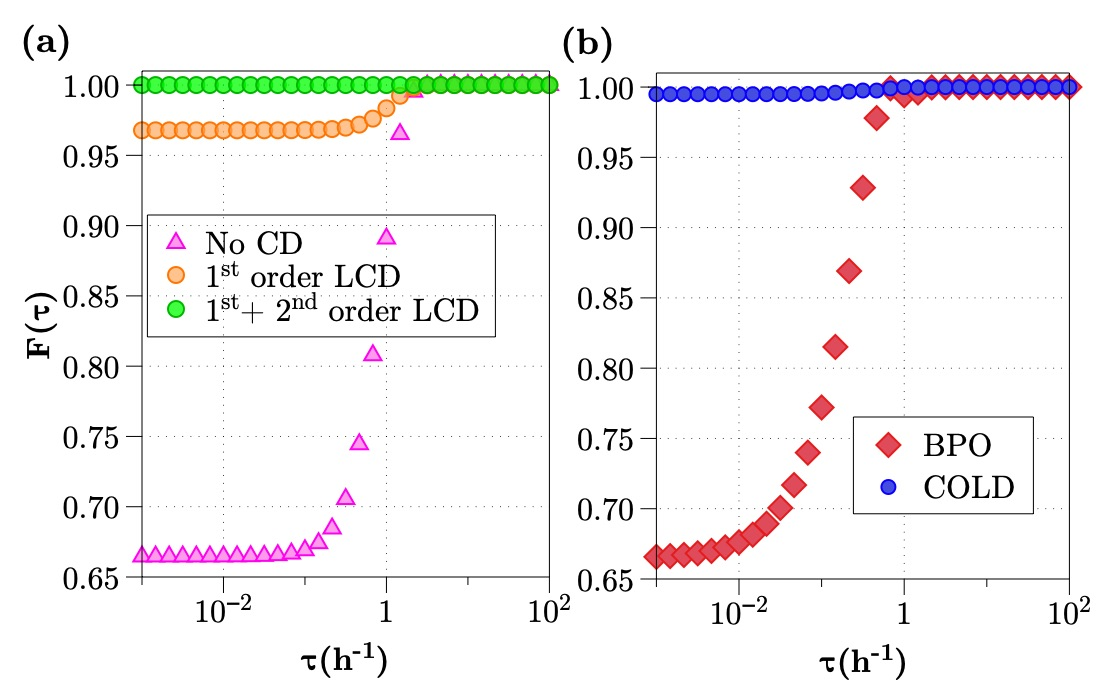
\includegraphics[width=0.8\linewidth]{images/twospins_fidelities.jpg} \caption[COLD applied to two-spin annealing]{}\label{fig:twospin_fidelities}
\end{figure}

\section{Ising chain}\label{sec:5.2_Ising_chain}

\begin{equation}\label{eq:ising_chain_hamiltonian}
    H_0(\lambda) = - J \sum_{j}^{N-1} \sz_j \sz_{j+1} + Z_0\sum_j^N \sz_j + \lambda X_f \sum_j^N \sx_j,
\end{equation}

\begin{equation}
    \AGP{\lambda}^{(1)} = \alpha \sum_{j}^N\sy_j,
\end{equation}

\begin{equation}
    \alpha(\lambda) = \frac{1}{2} \frac{Z_0 X_f}{Z_0^2 + \lambda^2 X_f^2 + 2J^2}.
\end{equation}

\begin{equation}
    \AGP{\lambda}^{(2)} = \alpha \sum_{j} \sy_j + \gamma  \sum_{j} (\sx_j \sy_{j+1} + \sy_j \sx_{j+1}) +  \zeta \sum_{j} (\sz_j \sy_{j+1} + \sy_j \sz_{j+1}) ,
\end{equation}

\section{Transport in a synthetic lattice}

\begin{figure}[t]
    \centering
    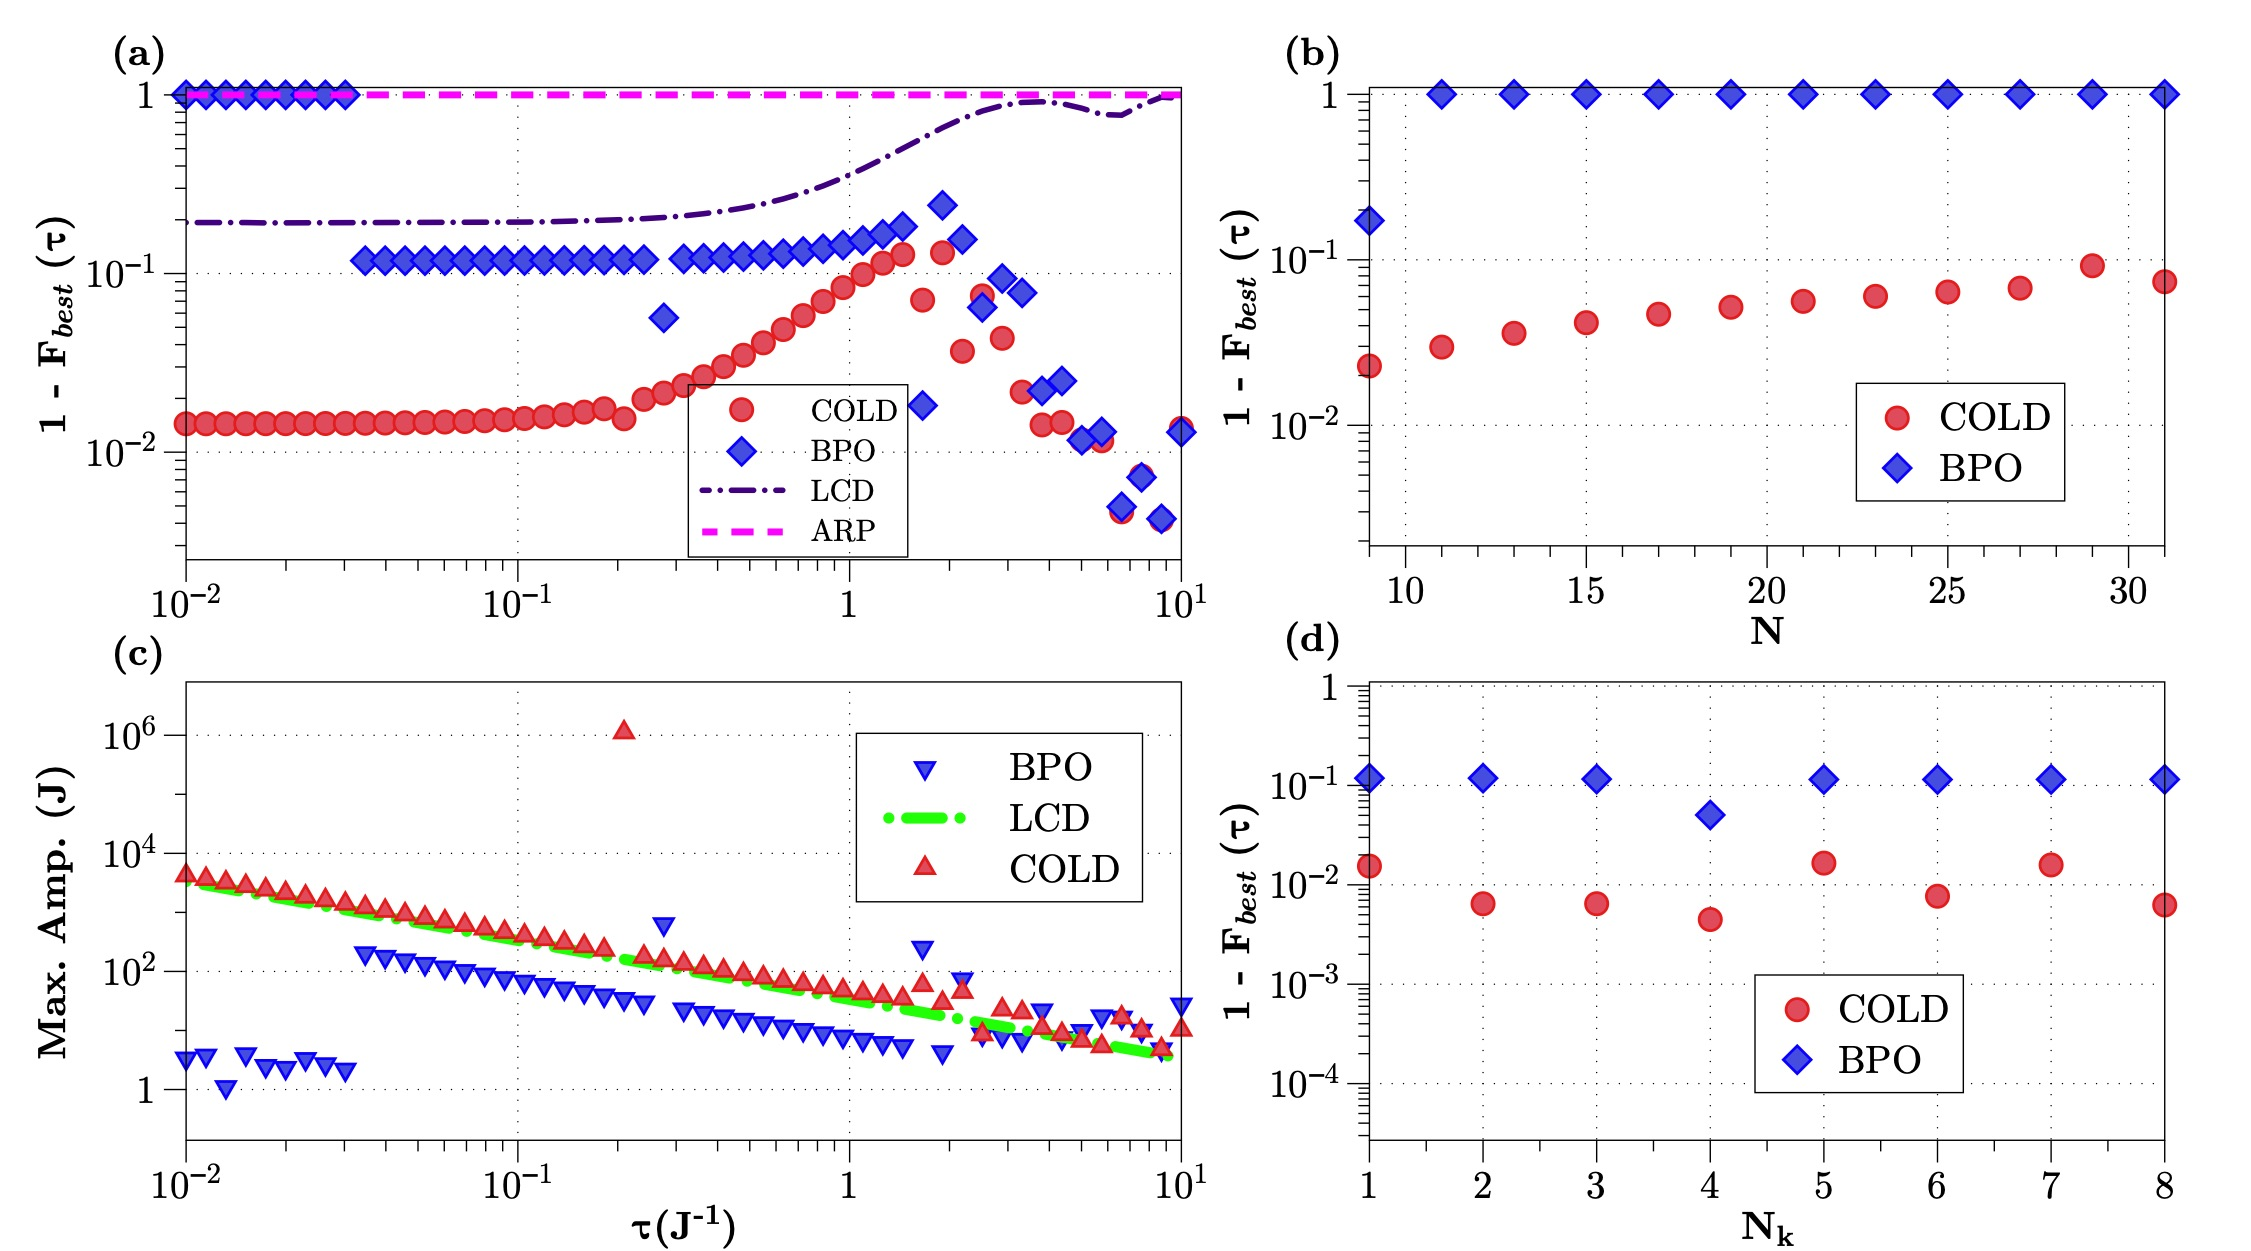
\includegraphics[width=\linewidth]{images/synthetic_lattice.jpg} \caption[COLD plots for ARP transport in a synthetic lattice]{}\label{fig:synthetic_results}
\end{figure}

The efficient transfer of states between opposite ends of a lattice could have future applications in the settings of quantum computation and simulation due to its promise of efficient transport of information \cite{lang_topological_2017}. This objective is often tackled in the setting of ultracold atoms in optical lattices. While the problem can be tuned to be a single-particle system and the analytical solutions of the corresponding instantaneous Schr\"odinger equation are known \cite{hatsugai_chern_1993,hugel_chiral_2014} even for a finite system \cite{duncan_exact_2018}, efficient evolution for state transfer is not straight-forward.  This is due to the fact that the majority of the states are delocalised across the lattice, meaning that the $\ket{\psi}\bra{\psi}$ terms of the CD Hamiltonian of Eq.~\eqref{eq:CD_Hamiltonian} are global in reach. It is common to consider this system in the tight-binding limit where the implementation of global terms is not straightforward. Such terms can be generated via the interactions of the atoms with cavity modes \cite{landig_quantum_2016,keller_phases_2017} or from dipolar interactions \cite{baranov_ultracold_2002, trefzger_ultracold_2011}. However, it would be ambitious to expect this control to be general enough to implement the CD Hamiltonian of the exact solutions.  This is one of the reasons that LCD has been pursued in this setting. 

Recently, LCD has been successfully applied to improve an adiabatic rapid passage (ARP) protocol for population transfer across a synthetic lattice \cite{meier_counterdiabatic_2020}. In this realisation, population transfer was achieved in a synthetic tight-binding lattice of laser coupled atomic momentum states. We will consider the same problem as in Ref.~\cite{meier_counterdiabatic_2020} but with the improvement that can be gained by COLD. This system is described by the Hamiltonian
\begin{equation}\label{eq:lattice_hamiltonian}
    H_0(t) = - \sum_n J_n(t)(c_n^{\dag}c_{n+1} + H.c.) + \sum_n V_n(t) c_n^{\dag}c_n,
\end{equation}

\begin{align} \label{eq:J_lattice}
    J_n(t) &= J_0(1.1 - \lambda) \\ \label{eq:V_lattice}
    V_n(t) &= n V_0 2 (\lambda - 1/2),
\end{align}

\begin{equation}\label{eq:tunneling}
    J_n(t) \rightarrow J_{n, \mathrm{CD}}(t) e^{-i\phi_{n, \mathrm{CD}}(t)},
\end{equation}
where
\begin{align}\label{eq:J_cd}
    J_{n, \mathrm{CD}}(t) = \sqrt{J_n(t)^2 + (\alpha_n(t)/\tau)^2}, \\ \label{eq:phi_cd}
    \phi_{n, \mathrm{CD}}(t)  = \arctan\left(-\frac{J_n(t)\tau}{\alpha_n(t)}\right),
\end{align}

\section{Preparing GHZ states in a system of frustrated spins}\label{sec:6.4_ghz_states}

\begin{figure}[t]
    \centering
    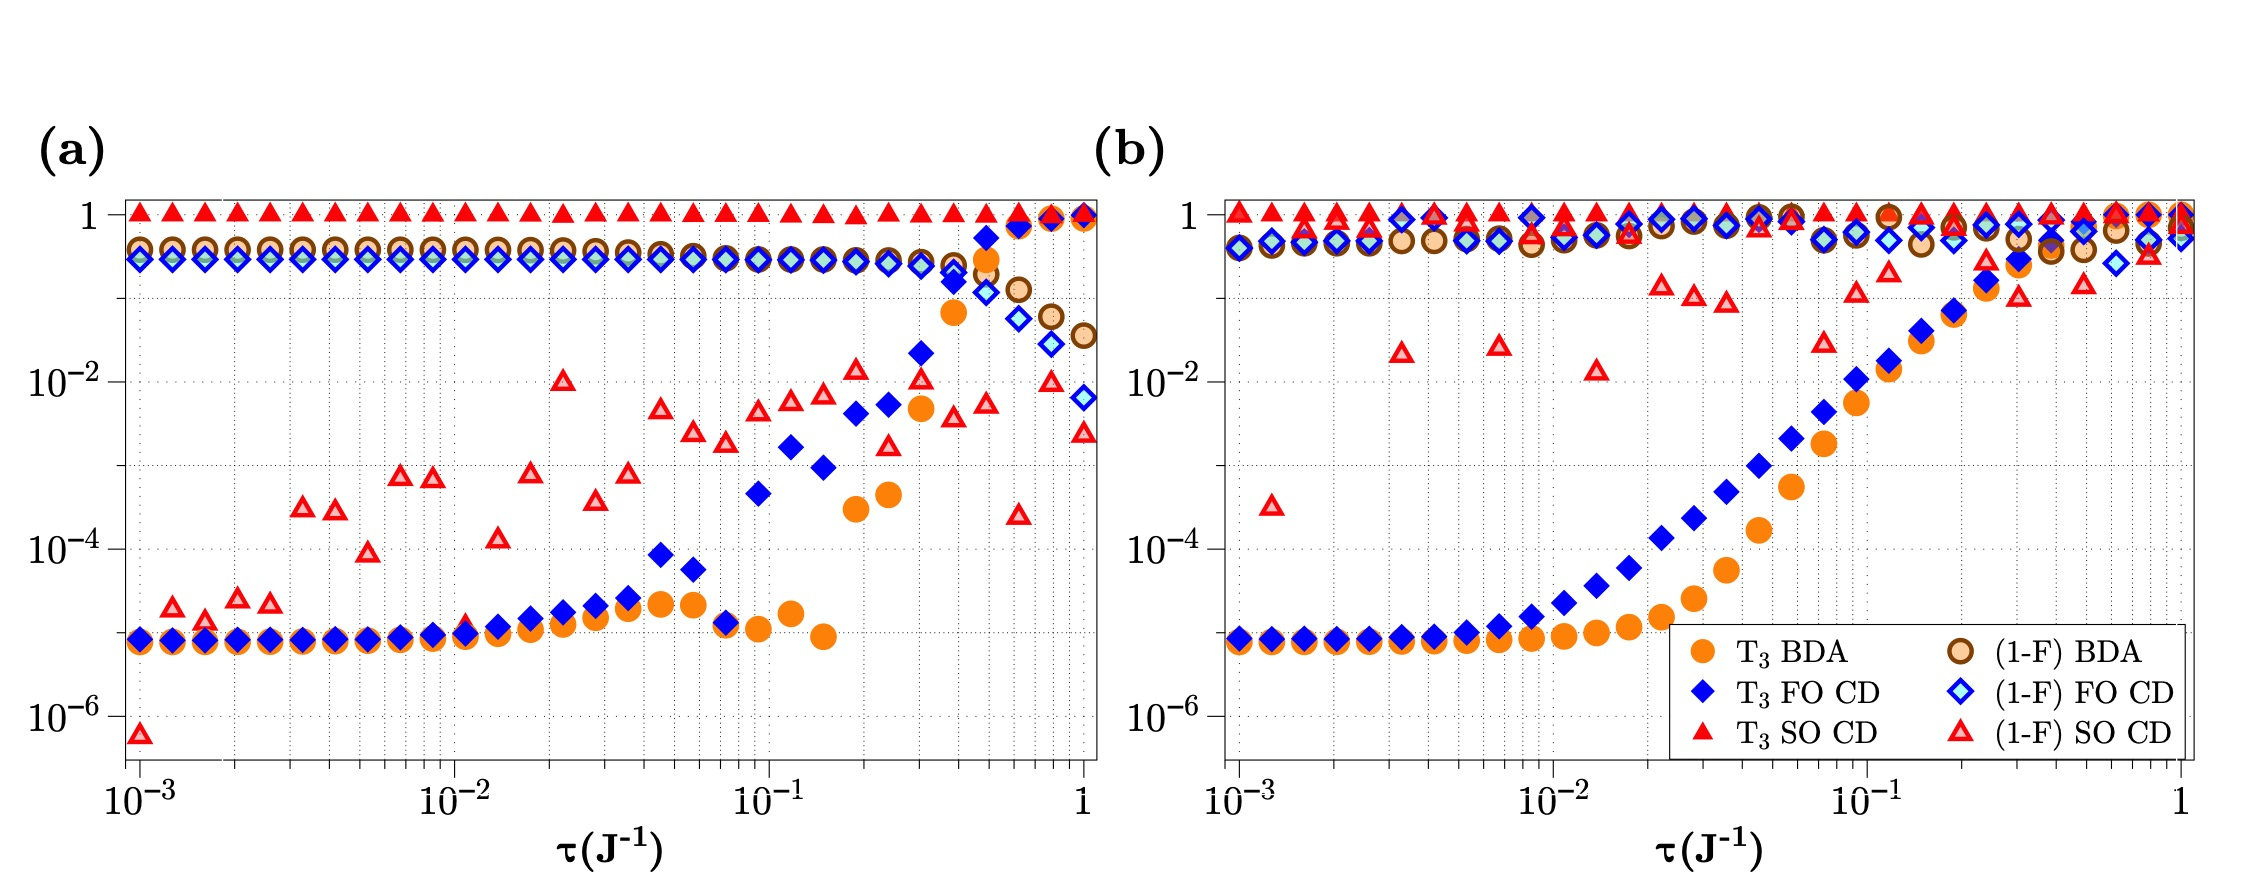
\includegraphics[width=\linewidth]{images/tangle_plots.jpg} \caption[Plots of entanglement and fidelity of GHZ states]{Plots of $T_3$ (Eq.~\eqref{eq:3-tangle}, solid shapes) and fidelity $(1 - F)$ with respect to the GHZ state (outlined shapes) of the final state prepared after optimising a GRAPE pulse with $N_k = 4$ parameters for each value of $\tau$.  (a) Optimisation is performed using $(1 - F)$ as the cost function}\label{fig:tangle_v_fidelity}
\end{figure}

Multipartite entanglement is a powerful resource for quantum computing and more broadly in quantum technologies, offering unique capabilities for information processing, secure communication, high-precision measurements, and understanding the foundations of quantum mechanics. An example of such highly entangled states is the GHZ (Greenberger–Horne–Zeilinger) state \cite{greenberger_bells_1990} on $N > 1$ spins:
\begin{equation}\label{eq:GHZ_state}
    \ket{\rm GHZ} = \frac{1}{\sqrt{2}} (\ket{0}^{\otimes N} + \ket{1}^{\otimes N}).
\end{equation}

\subsection{Tripartite GHZ entanglement}

The GHZ state exhibits a particular type of entanglement: when one of the subsystems is measured, the rest are no longer entangled and collapse into a product state. This is different to the other canonical type of multipartite entanglement exhibited by the W state \cite{cabello_bells_2002}, which for 3 spins can be written as:
\begin{equation}\label{eq:W_state}
    \ket{W} = \frac{1}{\sqrt{3}}(\ket{001} + \ket{010} + \ket{100}).
\end{equation}


GHZ states can be prepared via an annealing schedule on a system of frustrated spins. 

\begin{equation}\label{eq:ghz_hamiltonian}
    H_0(\lambda) = - J \Big( \sum_{j}^{N-1} \sz_j \sz_{j+1} + \sum_{j}^{N-2} \sz_j \sz_{j+2} \Big) - h(1 - \lambda) \Big( \sum_j^N (\sz_j + \sx_j) \Big).
\end{equation}

When $J$ is positive, the ground state of $H_0(1)$ is the GHZ state of Eq.~\ref{eq:GHZ_state}, whereas when it is negative 

While measuring the entanglement of a multipartite system is not quite as simple as in the bipartite case, there exists a notion of entanglement for a system of three spins: namely, the three-tangle, first introduced in Ref.~\cite{coffman_distributed_2000}, which

\begin{equation}\label{eq:3-tangle}
	\begin{aligned}
		T_3(\ket{\psi}) &= 4 \left| d_1 - 2 d_2 + 4 d_3 \right|, \\
		d1 &= c^2_{000}c^2_{111} + c^2_{001}c^2_{110} + c^2_{010}c^2_{101} + c^2_{011}c^2_{100}, \\
		d_2 &= c_{000}c_{001}c_{110}c_{111} + c_{000}c_{010}c_{101}c_{111} + c_{000}c_{011}c_{100}c_{111} \\
		 &+ c_{001}c_{010}c_{101}c_{110} + c_{001}c_{011}c_{100}c_{110} + c_{010}c_{011}c_{100}c_{101} \\
		d_3 &= c_{000}c_{110}c_{101}c_{011} + c_{100}c_{010}c_{001}c_{111}
	\end{aligned}
\end{equation}

Not the first time this is attempted with \acrref{CD}. \cite{sun_optimizing_2022}.

\section{Spin-1/2 XXZ chains of ultracold atoms}

The system is a Mott insulator of $^7$Li atoms in an optical lattice. With one particle per site and two hyperfine states, it realizes the (anisotropic) spin-1/2 Heisenberg model, where effective spin-spin interactions between neighboring sites are realized by a second-order tunneling process (superexchange) \cite{altman03, ddl03}. We apply a microwave field coupling the two hyperfine states with detuning $\delta = \omega - \omega_0$, where $\hbar \omega_0$ is the energy difference between the two hyperfine states and $\omega$ is the frequency of the microwave field, and with Rabi frequency $\Omega$. This is equivalent to having a z- and an x- magnetic field in a spin system respectively, realizing the anisotropic spin-1/2 Hamiltonian with external fields:
\begin{align}
H = & J_z \sum_{\langle i,j \rangle} S_i^zS_j^z+ J_{xy} \sum_{\langle i,j \rangle}  \left(S_i^xS_j^x + S_i^yS_j^y \right) \nonumber \\
& + \delta(\lambda) \sum_i S_i^z + \Omega(\lambda) \sum_i S_i^x,
\label{Heisenberg}
\end{align}
\chapter{Higher order AGP as a cost function}\label{chap:7_higher_order_agp}

\section{Return to two-spin annealing}

Hey there's lots of cool stuff to see here! Check out Appendix \ref{app:higher_order_AGP} for more nice plots and things. I might just keep the stuff in Fig.~\ref{fig:two_spin_higher_order} for now to keep it focused.

\begin{figure}[h]
    \centering
    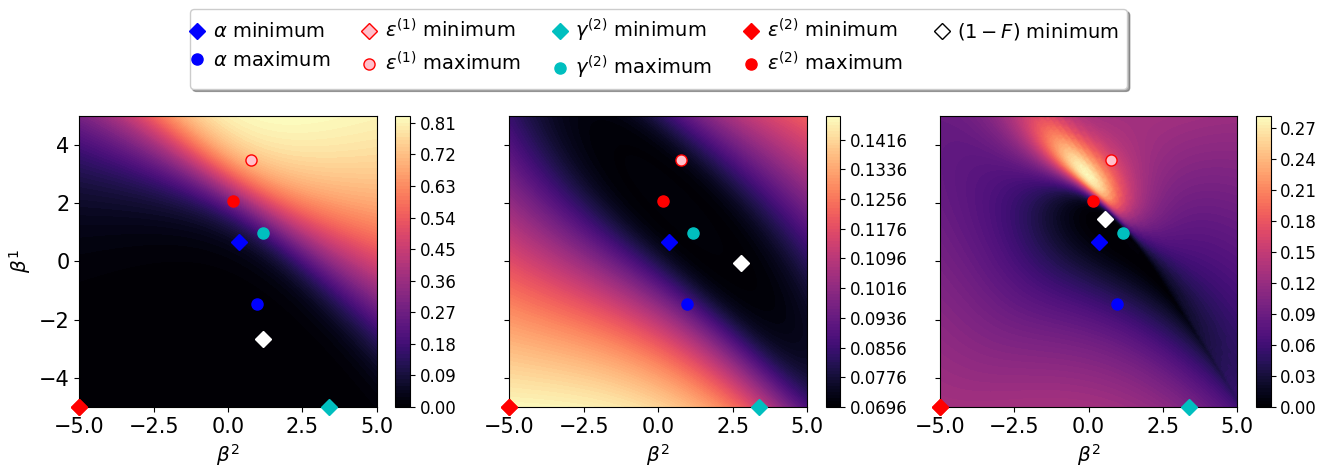
\includegraphics[width=\linewidth]{images/2spin_Integrals_scaled_by_norm_final.png} \caption[Two-spin annealing fidelity contour plots]{Current placeholder for final figure. (a) Only first order CD is applied. (b) only $\sz\sy, \sy\sz$ terms are applied. (c) All second-order terms are applied ($\sz\sy, \sy\sz$, $\sx\sy, \sy\sx$).}\label{fig:two_spin_higher_order}
\end{figure}

\section{GHZ states, fidelity and entanglement}

\begin{figure}[t]
    \centering
    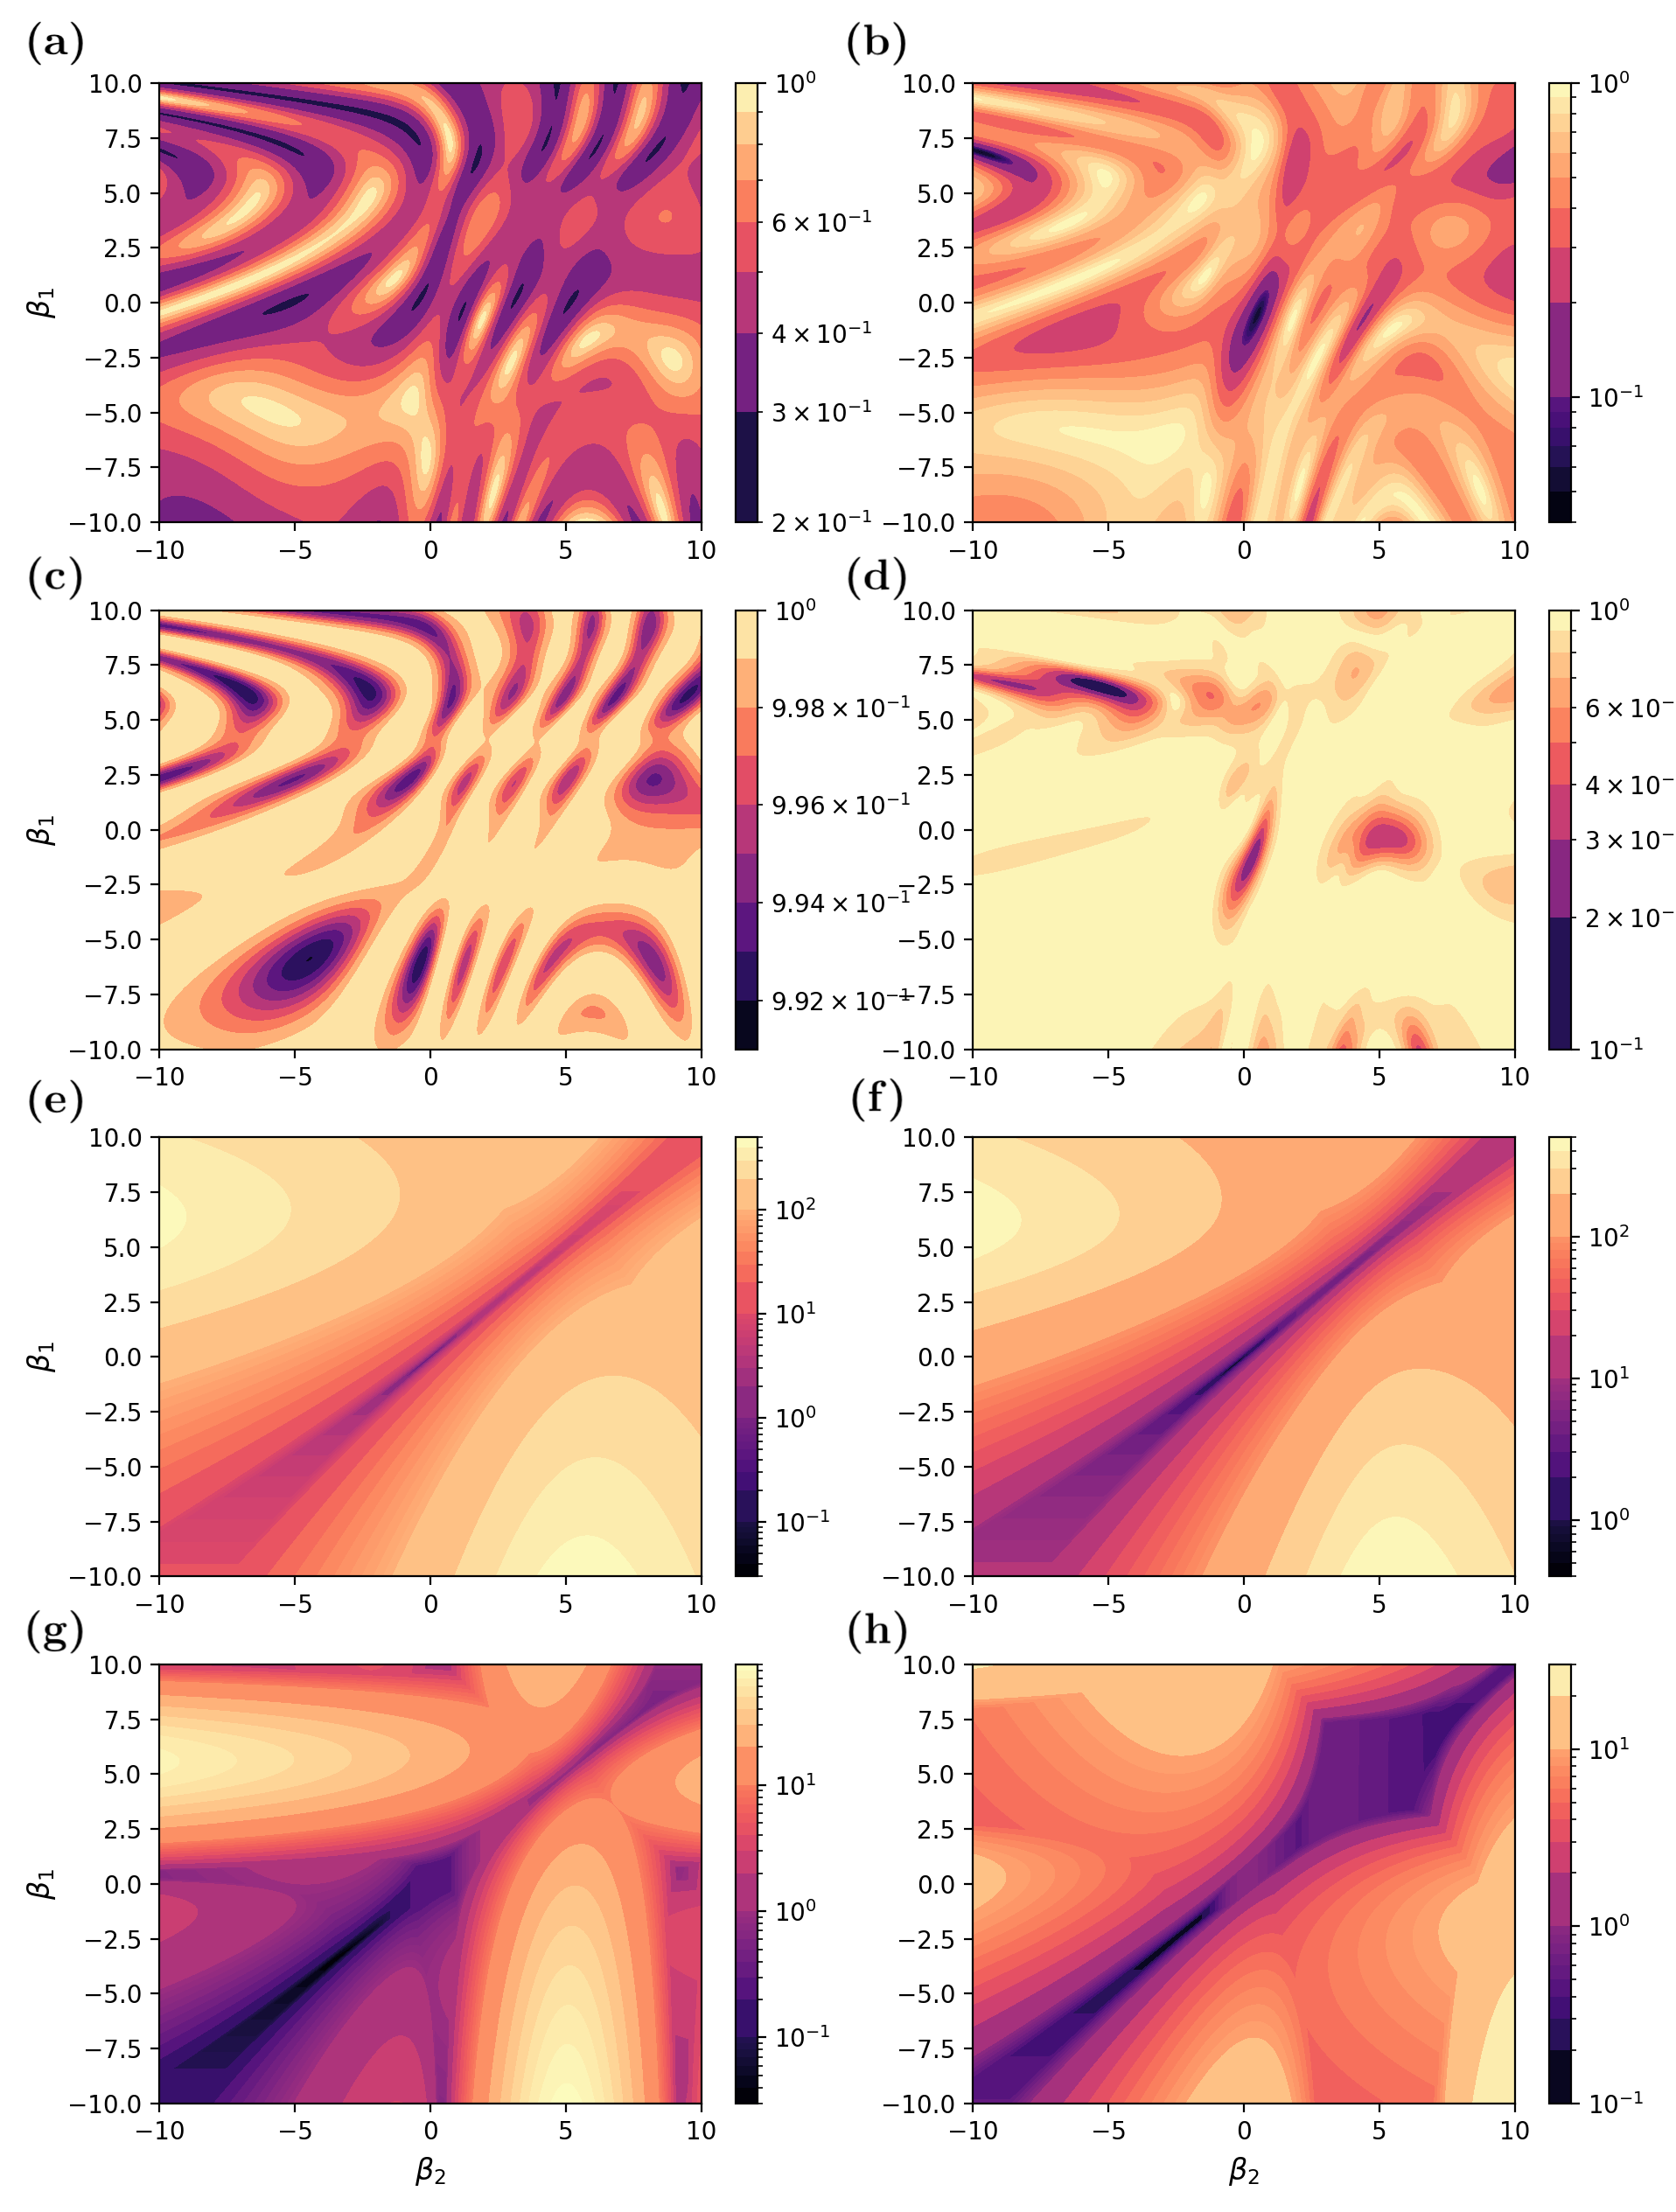
\includegraphics[width=\linewidth]{images/ghz_contour_plots.png} \caption[Contour plots of cost function landscapes for GHZ state preparation in frustrated spin systems.]{Contour plots, $\tau = 0.1 J^{-1}$, \acrref{GRAPE} for parameters $\beta_1$ and $\beta_2$. (a) FO CD infidelity, (b) SO CD infidelity, (c) FO CD $1 - T_3$, (d) SO CD $1 - T_3$, (e) FO CD amps ($\alpha$), (f) SO CD amps ($\alpha$) (g) SO CD amps ($\gamma$) (h) SO CD amps ($\zeta$)}\label{fig:two_spin_higher_order}
\end{figure}
\chapter{Conclusion}

%%%%%%%%%%%%%%%%%%%%%%%%%%%%%%%%%%%%%%%%%%%%%%%%%%%%%%%%%%%%%%
\appendix

\chapter{Rotating spin Hamiltonian}\label{app:rotating_spin_hamiltonian}

In Chap.~\ref{chap:2_adiabaticity} we used the example of a spin rotating in a magnetic field to illustrate adiabatic processes in quantum systems. We considered a spin starting in the $\ket{+}$ state and being rotated from the $x$ direction to the $z$ direction during some total time $\tau$ according to the Hamiltonian in Eq.~\eqref{eq:rotating_spin_H}, which I will reproduce here for convenience:
\begin{equation}\label{eq:rotating_spin_H_lambda}
    H(\lambda) = -\cos(\lambda)\sx - \sin(\lambda)\sz,
\end{equation}
with $\lambda(t) = \frac{\pi t}{2 \tau}$.

\chapter{Pontryagin maximum principle}\label{app:PMP}

\newtheorem{theorem}{Theorem}

\begin{theorem}[\acrref{PMP} for Mayer problems]\label{thm:pmp}
    For fixed final time $\tau$ and free final state assume $u$ is the optimal control and $x$ the corresponding trajectory solution of Eq.~\eqref{eq:control_ODE}. Then, there exists a nonzero vector $\lambda$ solution of the adjoint equations
  \begin{equation}
      \dotlambda^T = - \lambda^T f(x(t), u(t))
  \end{equation}
  with terminal condition
  \begin{equation}
      \lambda^T(\tau) = -\phi(x(\tau))
  \end{equation}
  such that, for almost every $t \in (0, \tau]$, we have
  \begin{equation}\label{eq:pmp_maximisation}
      \lambda^T(t) f(x(t), u(t)) \geq \lambda^T(t) f(x(t), v)
  \end{equation}
  for every $v$ in the set of the admissible values for the control $U$. Furthermore, for every $t \in [0, \tau]$
  \begin{equation}\label{eq:pmp_constant}
      \lambda^T(t) f(x(t), u(t)) = c,
  \end{equation}
  for a constant $c$
\end{theorem}

Using this, one can then define the \emph{optimal control Hamiltonian}:
\begin{equation}
    h(\lambda, x, u) := \lambda^T(t) f(x, u).
\end{equation}
Now we can recast Eqs.~\eqref{eq:pmp_maximisation} and \eqref{eq:pmp_constant}:
\begin{equation}
    \begin{aligned}
        h(\lambda(t), x(t), u(t)) &= c \\
        h(\lambda, x, u) &\geq h(\lambda, x, v),
    \end{aligned}
\end{equation}
The solution will be of the form $u := u(x, \lambda)$ and it can be solved with the system of equations
\begin{equation}
    \begin{aligned}
        \dot{x} &= f(x, u(x, \lambda)), \\
        \dotlambda^T &= -\lambda^T f(x, u(x, \lambda))
    \end{aligned}
\end{equation}
with the boundary conditions $x(0) = x_0$ and $\lambda^T(\tau) = -\phi(x(\tau))$. Every control which is obtained with this procedure satisfies the necessary conditions of optimality and it is a candidate to be the optimal control.

\chapter{Derivation of the CD coefficients for an arbitrary Ising graph}\label{app:arbitrary_ising_derivation}

An Ising Hamiltonian for $N$ spins and with both a transverse and longitudinal field can be written as:
\begin{equation}\label{eq:ising_hamiltonian}
    H(\lambda) = \sum_{i = 1}^{N-1}\sum_{j = i+1}^{N} J_{ij}(\lambda) \sz_i \sz_j + \sum_{i = 1}^{N} \Big( X_i(\lambda) \sx_i + Z_i(\lambda) \sz_i \Big)
\end{equation}
where the coefficients $J_{ij}$ correspond to couplings between spins $i$ and $j$. Systems like this can be viewed as undirected graphs, with each spin corresponding to a vertex and each coupling $J_{ij}$ denoting an edge between the corresponding spins. In the case of a weighted graph, the magnitude of each $J_{ij}$ can be viewed as the weight of the correspoding edge. This type of Hamiltonian, for specific values of $J_{ij}$, $X_i$ and $Z_i$ can be used to describe the two-spin annealing example of Sec.~\ref{sec:5.1_2spin_annealing}, the Ising chain from Sec.~\ref{sec:5.2_Ising_chain} and the frustrated spin model of Sec.~\ref{sec:}. 

The first order \acrref{LCD} ansatz is just single-spin operators:
\begin{equation}\label{eq:spin_agp_1storder}
    \AGP{\lambda}^{(1)} = \sum_{i = 1}^N \alpha_i(\lambda) \sy_i
\end{equation}
and the second order can be split up into 4 separate symmetries of operators:
\begin{equation}\label{eq:spin_agp_2ndorder}
        \AGP{\lambda}^{(2)} = \sum_{i = 1}^{N-1}\sum_{j = i+1}^{N} \Big( \gamma_{ij}(\lambda) \sx_i \sy_j + \Bar{\gamma}_{ij}(\lambda) \sy_i \sx_j + \zeta_{ij}(\lambda) \sz_i \sy_j + \Bar{\zeta}_{ij}(\lambda) \sy_i \sz_j \Big).
\end{equation}

What follows is a derivation that one might call `messy' on a good day. The first order commutators are computed as follows:
\begin{equation}\label{eq:first_order_AGP_commutator}
        i\comm{\alpha_i \sy_i}{H} = 2\alpha_i \Big[ \sum_{j = i+1}^{N} - J_{ij} \Big( \sx_i \sz_j + \sz_i \sx_j \Big) + X_i \sz_i - Z_i \sx_i \Big],
\end{equation}
where I have omitted the dependence on $\lambda$ of the terms. The second order expansions, sadly, look like this:
\begin{equation}
    \begin{aligned}
        i\comm{\gamma_{ij} \sx_i \sy_j}{H(\lambda)} &= 2\gamma_{ij} \Big[ \sum_{k = 1}^{i-1} (J_{ki} \sz_k \sy_i \sy_j - J_{kj} \sz_k \sx_i \sx_j)  + \sum_{k = i + 1}^{j-1} (J_{ik} \sy_i \sz_k \sy_j - J_{kj} \sx_i \sz_k \sx_j) \\ 
        &+ \sum_{k = j + 1}^N (J_{ik} \sy_i \sy_j \sz_k - J_{jk} \sx_i \sx_j \sz_k) + Z_i \sy_i \sy_j + X_j \sx_i \sz_j - Z_j \sx_i \sx_j \Big] \\
        i\comm{\Bar{\gamma}_{ij} \sy_i \sx_j}{H} &= 2\Bar{\gamma}_{ij} \Big[ \sum_{k = 1}^{i-1} (J_{kj} \sz_k \sy_i \sy_j - J_{ki} \sz_k \sx_i \sx_j) + \sum_{k = i + 1}^{j-1} (J_{kj} \sy_i \sz_k \sy_j - J_{ik} \sx_i \sz_k \sx_j) \\ 
        &+ \sum_{k = j + 1}^N (J_{jk} \sy_i \sy_j \sz_k - J_{ik} \sx_i \sx_j \sz_k)+ Z_j \sy_i \sy_j + X_i \sz_i \sx_j - Z_i \sx_i \sx_j \Big] \\ 
        i\comm{\zeta_{ij} \sz_i \sy_j}{H(\lambda)} &= 2\zeta_{ij} \Big[ -\sum_{k = 1}^{i-1} J_{kj} \sz_k \sz_i \sx_j - \sum_{k = i + 1}^{j-1} J_{kj} \sz_i \sz_k \sx_j - \sum_{k = j + 1}^N J_{jk} \sz_i \sx_j \sz_k  \\
        &- J_{ij} \sx_j - X_i \sy_i \sy_j + X_j \sz_i \sz_j - Z_j \sz_i\sx_j \Big] \\
        i\comm{\Bar{\zeta}_{ij} \sy_i \sz_j}{H(\lambda)} &= 2\Bar{\zeta}_{ij} \Big[ - \sum_{k = 1}^{i-1} J_{ki} \sz_k \sx_i \sz_j - \sum_{k = i + 1}^{j-1} J_{ik} \sx_i \sz_k \sz_j 
        - \sum_{k = j + 1}^N J_{ik} \sx_i \sz_j \sz_k \\
        &- J_{ij} \sx_i - X_j \sy_i \sy_j + X_i \sz_i \sz_j - Z_i \sx_i \sz_j \Big]
    \end{aligned}
\end{equation}
Combined, the above commutators along with the coefficients of $\dlambda H$ give the operator $G_{\lambda}(\AGP{\lambda}^{(1,2)})$ for an ansatz \acrref{AGP} constructed from both single- and two-spin operators (as per Eq.~\eqref{eq:G_operator}):
\begin{equation}\label{eq:ising_graph_G_operator}
    \begin{aligned}
        G_{\lambda}(\AGP{\lambda}^{(1,2)}) &= \sum_{i=1}^N \Bigg[ (\dot{X}_i - 2\alpha_i Z_i - 2\sum_{j=1}^{i-1} J_{ji}\zeta_{ji} - 2\sum_{j=i+1}^N J_{ij}\zetabar_{ij})\sx_i \\
        &+ (\dot{Z}_i + 2\alpha_i X_i)\sz_i \Bigg] \\
        &+ \sum_{i = 1}^{N-1} \sum_{j = i+1}^{N} \Bigg[(\dot{J}_{ij} + 2\zeta_{ij} X_j + 2\zetabar_{ij} X_i)\sz_i\sz_j \\
        &+ (2\gamma_{ij}Z_i + 2\gammabar_{ij} Z_j - 2 \zeta_{ij} X_i - 2 \zetabar_{ij} X_j)\sy_i\sy_j \\
        &+ (2\gamma_{ij}Z_j + 2\gammabar_{ij} Z_i)\sx_i\sx_j \\
        &+ (-2\alpha_i J_{ij} + 2\gamma_{ij}X_j - 2\zetabar_{ij} Z_i)\sx_i\sz_j \\
        &+ (-2\alpha_j J_{ij} + 2\gammabar_{ij}X_i - 2\zeta_{ij} Z_j)\sz_i\sx_j \\
        &+ \sum_{k = 1}^{i-1} \Big[ (2\gamma_{ij}J_{ki} + 2\gammabar_{ij} J_{kj})\sz_k\sy_i\sy_j + (2\gamma_{ij}J_{kj} + 2\gammabar_{ij} J_{ki})\sz_k\sx_i\sx_j \\
        &+ (- 2 \zeta_{ij} J_{kj} - 2 \zeta_{kj}J_{ij})\sz_k\sz_i\sx_j \Big] \\
        &+ \sum_{k = i+1}^{j-1} \Big[ (2\gamma_{ij}J_{ik} + 2\gammabar_{ij} J_{kj})\sy_i\sz_k\sy_j + (2\gamma_{ij}J_{kj} \\
        &+ 2\gammabar_{ij} J_{ik})\sx_i\sz_k\sx_j + (- 2 \zetabar_{ij} J_{ik} - 2 \zeta_{ik}J_{ij})\sz_k\sx_i\sz_j \Big] \\
        &+ \sum_{k = j+1}^N \Big[ (2\gamma_{ij}J_{ik} + 2\gammabar_{ij} J_{jk})\sy_i\sy_j\sz_k + (2\gamma_{ij}J_{jk} + 2\gammabar_{ij} J_{ik})\sx_i\sx_j\sz_k \\
        &+ (- 2 \zetabar_{ij} J_{ik} - 2 \zetabar_{ik}J_{ij})\sz_i\sx_j\sz_k \Big] \Bigg].
    \end{aligned}
\end{equation}
In order to find the coupled set of equations that allow us to compute each of the coefficients in the approximate \acrref{AGP} according to the \acrref{LCD} approach, we need to minimise the action $\mathcal{S} = \Tr[G_{\lambda}^2]$ with respect to each of the coefficients. As the Pauli operators and their tensor products are traceless, this means that the action is merely the sum of the squares of all the orthogonal operator coefficients of $G_{\lambda}$. Minimising $\mathcal{S}$ with respect to each $\alpha_i$ gives:
\begin{equation}\label{eq:ising_graph_minimise_alpha}
    \begin{aligned}
        &\alpha_i \Big[2Z_i^2 + 2X_i^2 + \sum_{j = 1}^{i-1}2J_{ji}^2 + \sum_{i+1}^{N}2J_{ij}^2 \Big] \\
        \sum_{j = i+1}^N &\gamma_{ij} \Big[ -2J_{ij}X_j \Big] + \sum_{j = 1}^{i-1} \gammabar_{ji} \Big[ -2J_{ji}X_j \Big] \\
        \sum_{j = i+1}^N &\zetabar_{ij} \Big[ 4J_{ij}Z_i \Big] + \sum_{j = 1}^{i-1} \zeta_{ji} \Big[4 J_{ji}Z_i \Big] \\
        &= Z_i \dot{X}_i - X_i \dot{Z}_i,
    \end{aligned}
\end{equation}
where $i$ is fixed. Fixing $i$ and $j$ and minimising with respect to each $\gamma_{ij}$ gives:
\begin{equation}\label{eq:ising_graph_minimise_gamma}
    \begin{aligned}
        &\alpha_i\Big[ -X_j J_{ij} \Big] + \zeta_{ij}\Big[ -  X_i Z_i\Big] + \zetabar_{ij} \Big[ -2 X_j Z_i \Big] \\
        + \: &\gamma_{ij} \Big[ Z_i^2 + Z_j^2 + X_j^2 + \sum_{k = 1}^{i-1} (J_{ki}^2 + J_{kj}^2) + \sum_{k = i+1}^{j-1} (J_{ik}^2 + J_{kj}^2) + \sum_{k = j+1}^N (J_{ik}^2 + J_{jk}^2) \Big] \\
        + \: &\gammabar_{ij} \Big[ 2 Z_i Z_j + \sum_{k = 1}^{i-1} 2J_{ki}J_{kj} + \sum_{k = i+1}^{j-1} 2J_{ik}J_{kj} + \sum_{k = j+1}^N 2J_{ik}J_{jk} \Big] = 0
    \end{aligned}
\end{equation}
and likewise for each $\gammabar$:
\begin{equation}\label{eq:ising_graph_minimise_gammabar}
    \begin{aligned}
        &\alpha_j\Big[ -X_i J_{ij} \Big] + \zeta_{ij}\Big[ - 2 X_i Z_j\Big] + \zetabar_{ij} \Big[ - X_j Z_j \Big] \\
        + \: &\gammabar_{ij} \Big[ Z_i^2 + Z_j^2 + X_i^2 + \sum_{k = 1}^{i-1} (J_{ki}^2 + J_{kj}^2) + \sum_{k = i+1}^{j-1} (J_{ik}^2 + J_{kj}^2) + \sum_{k = j+1}^N (J_{ik}^2 + J_{jk}^2) \Big] \\
        + \: &\gamma_{ij} \Big[ 2 Z_i Z_j + \sum_{k = 1}^{i-1} 2J_{ki}J_{kj} + \sum_{k = i+1}^{j-1} 2J_{ik}J_{kj} + \sum_{k = j+1}^N 2J_{ik}J_{jk} \Big] = 0.
    \end{aligned}
\end{equation}
Finally, for fixed $i$, $j$, we minimise with respect to $\zeta_{ij}$:
\begin{equation}\label{eq:ising_graph_minimise_zeta}
    \begin{aligned}
        &\alpha_j\Big[ 4 Z_j J_{ij} \Big] + \gamma_{ij}\Big[ - 2 X_i Z_i\Big] + \gammabar_{ij} \Big[ - 4 X_i Z_j \Big] \\
        + \: &\zeta_{ij} \Big[ 2 Z_j^2 + 2X_i^2 + 2X_j^2 + \sum_{k = 1}^{i-1} 2 J_{kj}^2 + \sum_{k = i+1}^{j-1} 2 J_{jk}^2 \Big] + \zetabar_{ij}\Big[ 4 X_i X_j \Big] \\
        + \sum_{k = 1}^{i-1} &\zeta_{kj}\Big[ 2 J_{ij} J_{kj} \Big] + \sum_{k = 1}^{j-1} \zeta_{kj} \Big[2 J_{ij}J_{kj}\Big] \\
        + \sum_{k = i +1}^{j-1} &\zetabar_{jk} 2 J_{ij} J_{jk} + \sum_{k = j +1}^N \zetabar_{jk} 2 J_{ij} J_{jk} = J_{ij} \dot{X}_j - \dot{J}_{ij} X_j
    \end{aligned}
\end{equation}
and with respect to $\zetabar_{ij}$:
\begin{equation}\label{eq:ising_graph_minimise_zetabar}
    \begin{aligned}
        &\alpha_i\Big[ 4 Z_i J_{ij} \Big] + \gamma_{ij}\Big[ - 4 X_j Z_i\Big] + \gammabar_{ij} \Big[ - 2 X_j Z_j \Big] \\
        + \: &\zetabar_{ij} \Big[ 2 Z_i^2 + 2X_i^2 + 2X_j^2 + \sum_{k = i+1}^{j-1} 2 J_{ik}^2 + \sum_{k = j+1}^N 2 J_{ik}^2 \Big] + \zeta_{ij}\Big[ 4 X_i X_j \Big] \\
        + \sum_{k = i+1}^N &\zetabar_{ik}\Big[ 2 J_{ij} J_{ik} \Big] + \sum_{k = j+1}^N \zetabar_{ik} \Big[2 J_{ij}J_{ik}\Big] \\
        + \sum_{k = 1}^{i-1} &\zeta_{ki} 2 J_{ij} J_{ki} + \sum_{k = i+1}^{j-1} \zeta_{ik} 2 J_{ij} J_{ik} = J_{ij} \dot{X}_i - \dot{J}_{ij} X_i.
    \end{aligned}
\end{equation}

Armed with this knowledge, we can now explore the non-adiabatic effects generated by one- and two-spin operators on any random time-dependent Ising graph Hamiltonian. 

\chapter{More details for the Ising spin chain}\label{app:ising}

\begin{figure}[h]
    \centering
    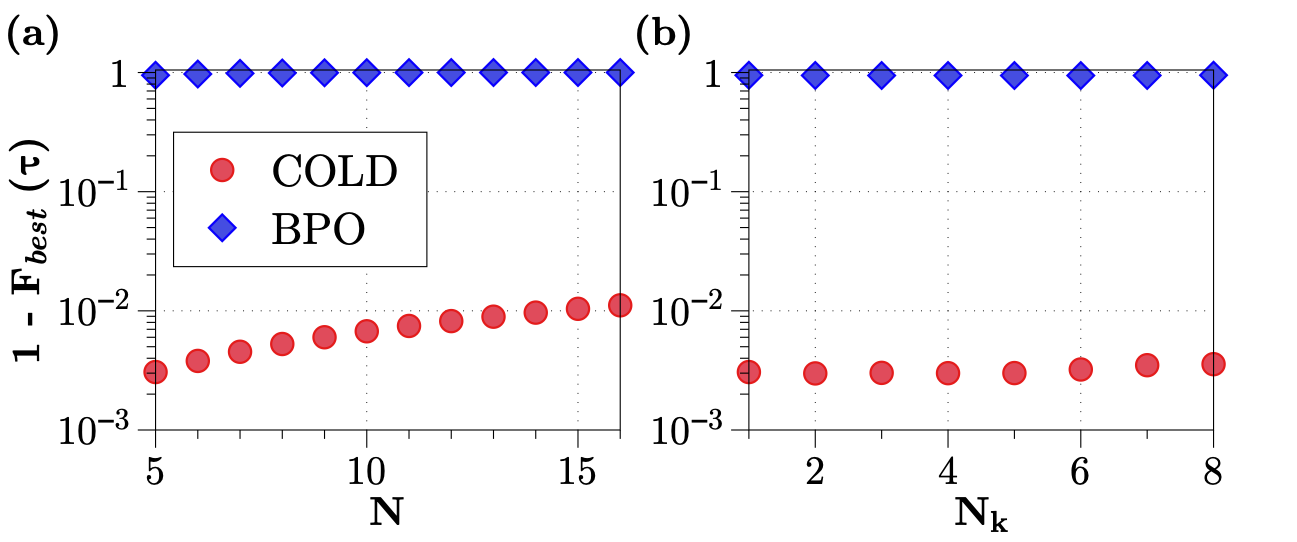
\includegraphics[width=0.8\linewidth]{images/ScalingN.png} \caption[Plots of how final state fidelities scale using COLD and BPO for different system sizes and optimisable parameters.]{Reproduced from \cite{cepaite_cold_2023}.}\label{fig:ising_maxamp}
\end{figure}

\begin{figure}[h]
    \centering
    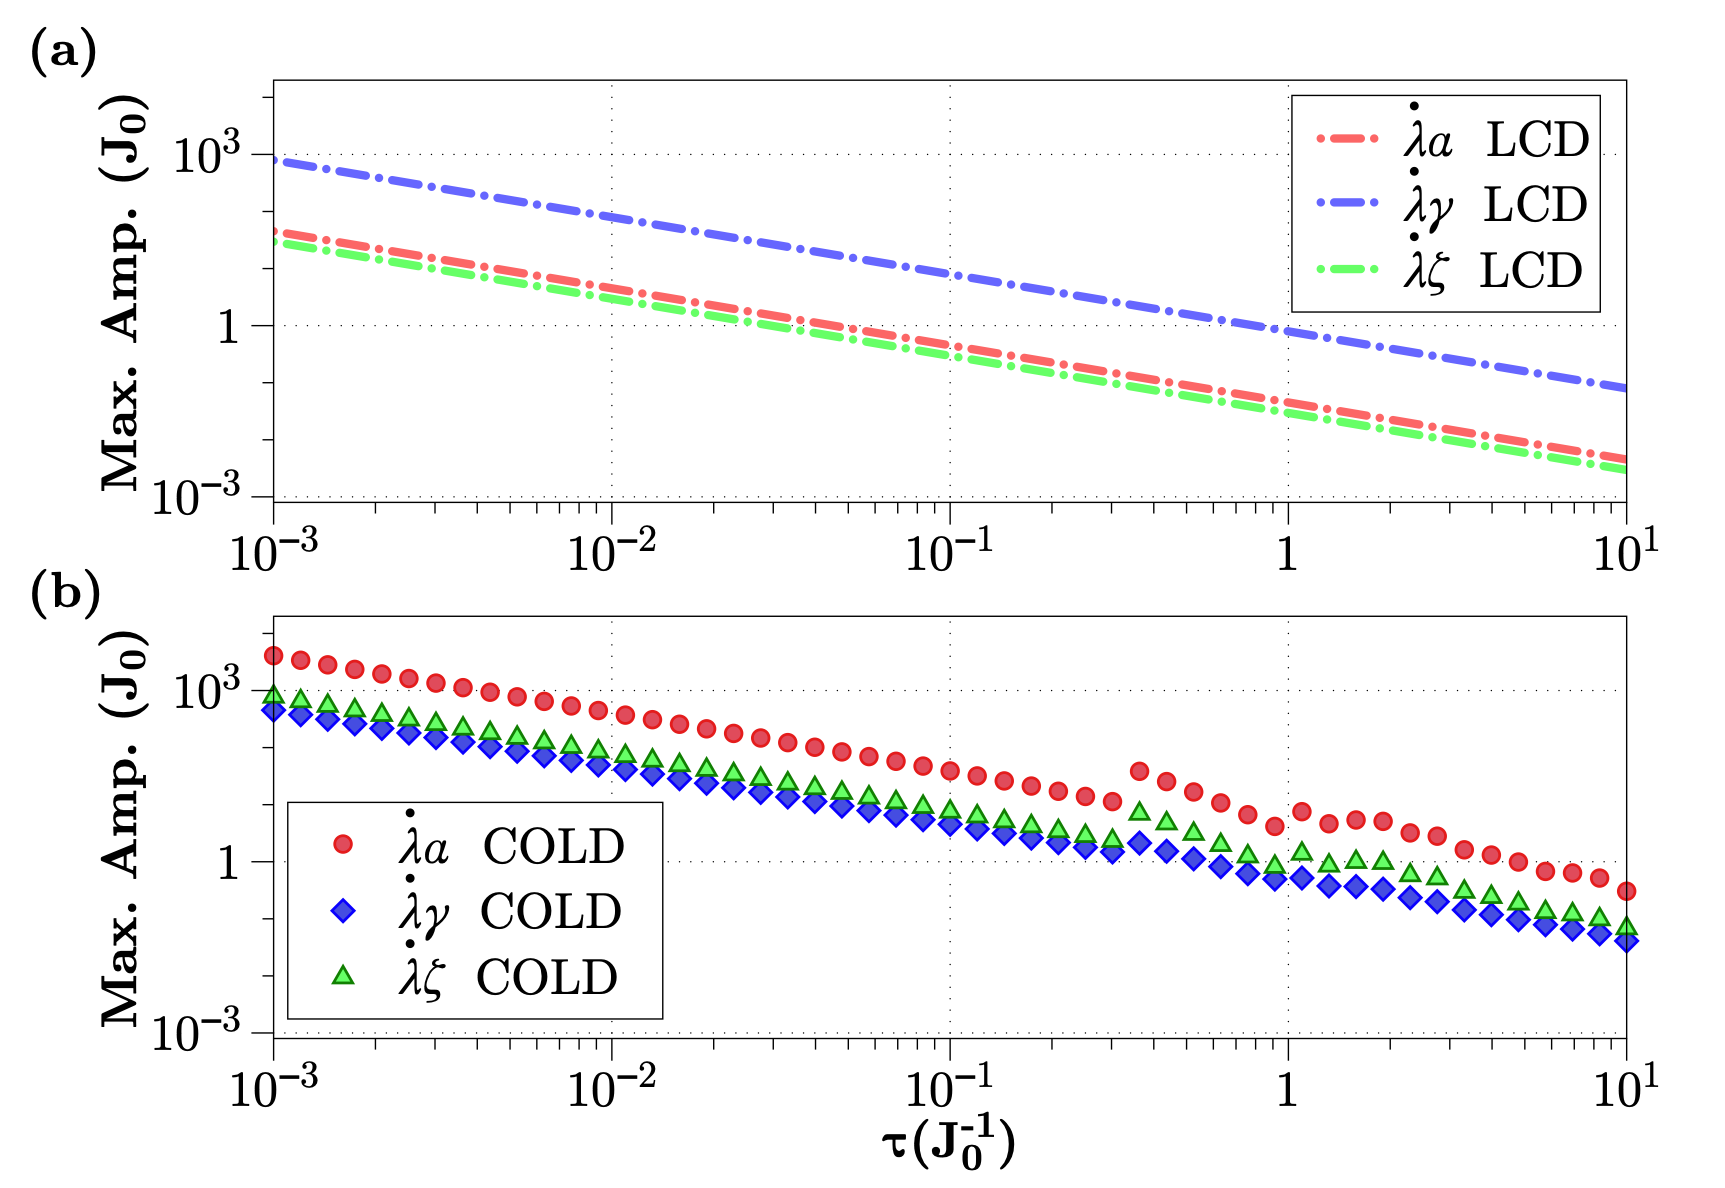
\includegraphics[width=0.8\linewidth]{images/MaxAmp.png} \caption[Plots of maximum amplitudes of LCD drives for the Ising spin chain.]{Reproduced from \cite{cepaite_cold_2023}.}\label{fig:ising_maxamp}
\end{figure}

\chapter{More details and plots for the higher order AGP chapter}\label{app:higher_order_AGP}

I have so much stuff to add here, might just leave some here for now. 


\begin{figure}[t]
\centering
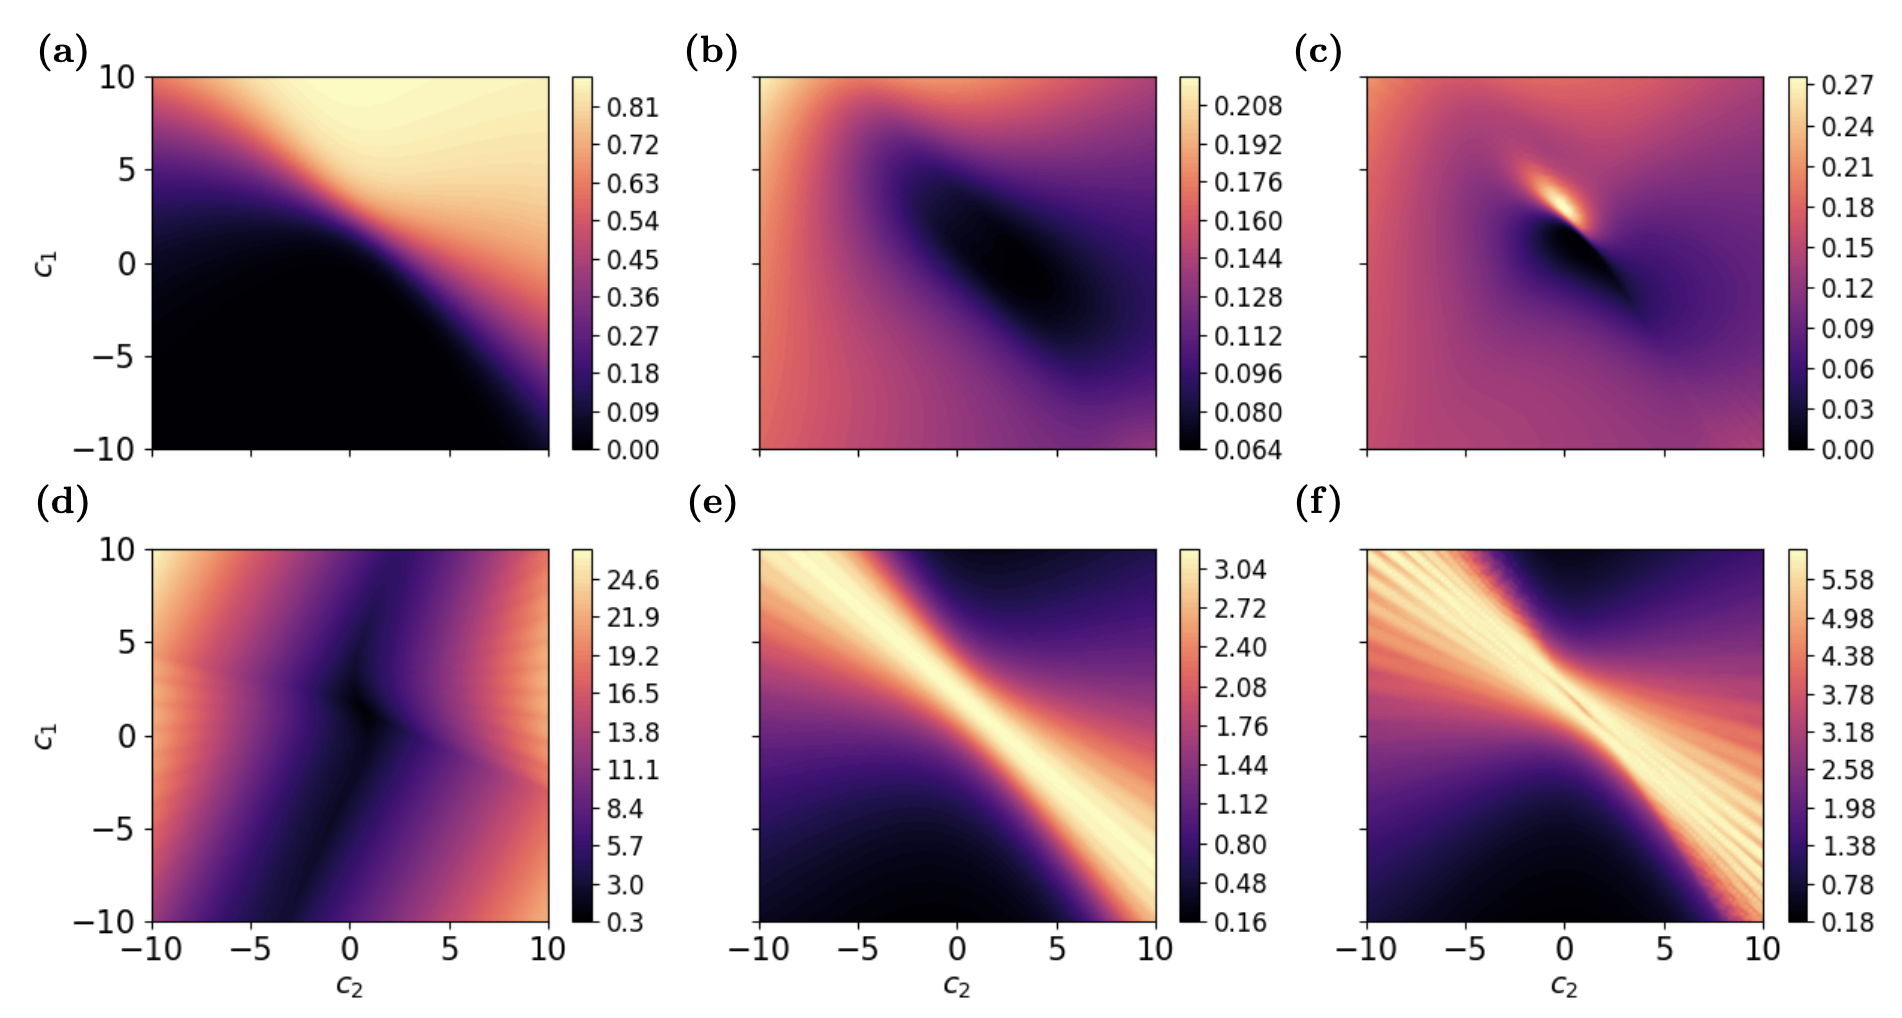
\includegraphics[width=\linewidth]{images/two_spin_contours_maxes.png} \caption{Placeholder: max amplitude scaled by Hamiltonian norm}\label{fig:}
\end{figure}


%%%%%%%%%%%%%%%%%%%%%%%%%%%%%%%%%%%%%%%%%%%%%%%%%%%%%%%%%%%%%%


%%%%%%%%%%%%%%%%%%%%%%%%%%%%%%%%%%%%%%%%%%%%%%%%%%%%%%%%%%%%%%
\addcontentsline{toc}{chapter}{Bibliography}
\bibliographystyle{util/ieeetran.bst}
\bibliography{references}

\end{document}